% Options for packages loaded elsewhere
\PassOptionsToPackage{unicode}{hyperref}
\PassOptionsToPackage{hyphens}{url}
\PassOptionsToPackage{dvipsnames,svgnames,x11names}{xcolor}
%
\documentclass[
  authoryear,
  preprint,
  3p,
  onecolumn]{elsarticle}

\usepackage{amsmath,amssymb}
\usepackage{iftex}
\ifPDFTeX
  \usepackage[T1]{fontenc}
  \usepackage[utf8]{inputenc}
  \usepackage{textcomp} % provide euro and other symbols
\else % if luatex or xetex
  \usepackage{unicode-math}
  \defaultfontfeatures{Scale=MatchLowercase}
  \defaultfontfeatures[\rmfamily]{Ligatures=TeX,Scale=1}
\fi
\usepackage{lmodern}
\ifPDFTeX\else  
    % xetex/luatex font selection
\fi
% Use upquote if available, for straight quotes in verbatim environments
\IfFileExists{upquote.sty}{\usepackage{upquote}}{}
\IfFileExists{microtype.sty}{% use microtype if available
  \usepackage[]{microtype}
  \UseMicrotypeSet[protrusion]{basicmath} % disable protrusion for tt fonts
}{}
\makeatletter
\@ifundefined{KOMAClassName}{% if non-KOMA class
  \IfFileExists{parskip.sty}{%
    \usepackage{parskip}
  }{% else
    \setlength{\parindent}{0pt}
    \setlength{\parskip}{6pt plus 2pt minus 1pt}}
}{% if KOMA class
  \KOMAoptions{parskip=half}}
\makeatother
\usepackage{xcolor}
\setlength{\emergencystretch}{3em} % prevent overfull lines
\setcounter{secnumdepth}{5}
% Make \paragraph and \subparagraph free-standing
\makeatletter
\ifx\paragraph\undefined\else
  \let\oldparagraph\paragraph
  \renewcommand{\paragraph}{
    \@ifstar
      \xxxParagraphStar
      \xxxParagraphNoStar
  }
  \newcommand{\xxxParagraphStar}[1]{\oldparagraph*{#1}\mbox{}}
  \newcommand{\xxxParagraphNoStar}[1]{\oldparagraph{#1}\mbox{}}
\fi
\ifx\subparagraph\undefined\else
  \let\oldsubparagraph\subparagraph
  \renewcommand{\subparagraph}{
    \@ifstar
      \xxxSubParagraphStar
      \xxxSubParagraphNoStar
  }
  \newcommand{\xxxSubParagraphStar}[1]{\oldsubparagraph*{#1}\mbox{}}
  \newcommand{\xxxSubParagraphNoStar}[1]{\oldsubparagraph{#1}\mbox{}}
\fi
\makeatother


\providecommand{\tightlist}{%
  \setlength{\itemsep}{0pt}\setlength{\parskip}{0pt}}\usepackage{longtable,booktabs,array}
\usepackage{calc} % for calculating minipage widths
% Correct order of tables after \paragraph or \subparagraph
\usepackage{etoolbox}
\makeatletter
\patchcmd\longtable{\par}{\if@noskipsec\mbox{}\fi\par}{}{}
\makeatother
% Allow footnotes in longtable head/foot
\IfFileExists{footnotehyper.sty}{\usepackage{footnotehyper}}{\usepackage{footnote}}
\makesavenoteenv{longtable}
\usepackage{graphicx}
\makeatletter
\newsavebox\pandoc@box
\newcommand*\pandocbounded[1]{% scales image to fit in text height/width
  \sbox\pandoc@box{#1}%
  \Gscale@div\@tempa{\textheight}{\dimexpr\ht\pandoc@box+\dp\pandoc@box\relax}%
  \Gscale@div\@tempb{\linewidth}{\wd\pandoc@box}%
  \ifdim\@tempb\p@<\@tempa\p@\let\@tempa\@tempb\fi% select the smaller of both
  \ifdim\@tempa\p@<\p@\scalebox{\@tempa}{\usebox\pandoc@box}%
  \else\usebox{\pandoc@box}%
  \fi%
}
% Set default figure placement to htbp
\def\fps@figure{htbp}
\makeatother

\usepackage{array,longtable}
\setlength{\LTleft}{0pt}
\setlength{\LTright}{0pt}
\makeatletter
\def\ps@pprintTitle{%
  \let\@oddhead\@empty
  \let\@evenhead\@empty
  \let\@oddfoot\@empty
  \let\@evenfoot\@empty}
\makeatother
\usepackage{newunicodechar}
\newunicodechar{≥}{\ensuremath{\geq}}
\newunicodechar{≤}{\ensuremath{\leq}}
\newunicodechar{≈}{\ensuremath{\approx}}
\newunicodechar{∼}{\ensuremath{\sim}} % Unicode "tilde operator"
\newunicodechar{×}{\ensuremath{\times}}
\newunicodechar{∈}{\ensuremath{\in}}
\newunicodechar{ρ}{\ensuremath{\rho}}
\makeatletter
\@ifpackageloaded{caption}{}{\usepackage{caption}}
\AtBeginDocument{%
\ifdefined\contentsname
  \renewcommand*\contentsname{Table of contents}
\else
  \newcommand\contentsname{Table of contents}
\fi
\ifdefined\listfigurename
  \renewcommand*\listfigurename{List of Figures}
\else
  \newcommand\listfigurename{List of Figures}
\fi
\ifdefined\listtablename
  \renewcommand*\listtablename{List of Tables}
\else
  \newcommand\listtablename{List of Tables}
\fi
\ifdefined\figurename
  \renewcommand*\figurename{Figure}
\else
  \newcommand\figurename{Figure}
\fi
\ifdefined\tablename
  \renewcommand*\tablename{Table}
\else
  \newcommand\tablename{Table}
\fi
}
\@ifpackageloaded{float}{}{\usepackage{float}}
\floatstyle{ruled}
\@ifundefined{c@chapter}{\newfloat{codelisting}{h}{lop}}{\newfloat{codelisting}{h}{lop}[chapter]}
\floatname{codelisting}{Listing}
\newcommand*\listoflistings{\listof{codelisting}{List of Listings}}
\makeatother
\makeatletter
\makeatother
\makeatletter
\@ifpackageloaded{caption}{}{\usepackage{caption}}
\@ifpackageloaded{subcaption}{}{\usepackage{subcaption}}
\makeatother

\usepackage[]{natbib}
\bibliographystyle{elsarticle-harv}
\usepackage{bookmark}

\IfFileExists{xurl.sty}{\usepackage{xurl}}{} % add URL line breaks if available
\urlstyle{same} % disable monospaced font for URLs
\hypersetup{
  pdftitle={Direct China/Hong Kong flights and Europe's first-wave COVID-19 excess mortality (2020): a EUROCONTROL ADRR coverage audit and exploratory analysis},
  pdfauthor={Maximilian Elixhauser},
  pdfkeywords={COVID‑19, Excess mortality, Air travel / international
flights, EUROCONTROL ADRR, Europe, Spearman rank correlation},
  colorlinks=true,
  linkcolor={blue},
  filecolor={Maroon},
  citecolor={Blue},
  urlcolor={Blue},
  pdfcreator={LaTeX via pandoc}}


\setlength{\parindent}{6pt}
\begin{document}

\begin{frontmatter}
\title{Direct China/Hong Kong flights and Europe's first-wave COVID-19
excess mortality (2020): a EUROCONTROL ADRR coverage audit and
exploratory analysis}
\author[1]{Maximilian Elixhauser%
\corref{cor1}%
}
 \ead{maximilian.elixhauser@stud.plus.ac.at} 

\affiliation[1]{organization={University of Salzburg},,postcodesep={}}

\cortext[cor1]{Corresponding author}

        
\begin{abstract}
We test whether direct long-haul exposure to China/Hong Kong just before
Europe's COVID-19 shutdown helps explain first-wave excess mortality.
Using EUROCONTROL's Aviation Data Repository for Research (ADRR), we
count inbound IFR passenger flights from Mainland China and Hong Kong in
December 2019 and March 2020 across 25 continental EUROCONTROL states (
\(F_{\text{DEC}}, F_{\text{MAR}}, F_{\text{SUM}}\) ). Outcomes are
excess deaths per million on 5 May in 2020--2023 (nearest value ±7 days;
Our World in Data / World Mortality Dataset). A coverage audit shows
that community ADS-B (OpenSky) undercounts CN/HK → Europe-25 arrivals,
so ADRR provides exposure while OpenSky is used only for QC. In 2020,
exposure is positively associated with excess mortality (Spearman
\(\rho = 0.526\); 95\% CI 0.177--0.771; \(p = 0.007\)); the top exposure
quartile recorded ≈ 465 more deaths per million than the bottom
quartile. The association weakens toward zero in 2021 and reverses in
2022 (negative and significant), remaining negative in 2023 with a 95\%
CI that includes zero. Limitations include the missing February ADRR
snapshot, lack of passenger-load information (``ghost flights''), and
unobserved multi-leg itineraries.
\end{abstract}





\begin{keyword}
    COVID‑19 \sep Excess mortality \sep Air travel / international
flights \sep EUROCONTROL ADRR \sep Europe \sep 
    Spearman rank correlation
\end{keyword}
\end{frontmatter}
    

\clearpage

\section{Glossary}\label{glossary}

\begin{longtable}[]{@{}
  >{\raggedright\arraybackslash}p{(\linewidth - 2\tabcolsep) * \real{0.3200}}
  >{\raggedright\arraybackslash}p{(\linewidth - 2\tabcolsep) * \real{0.6800}}@{}}
\caption{Glossary of acronyms and
symbols.}\label{tbl-glossary}\tabularnewline
\toprule\noalign{}
\begin{minipage}[b]{\linewidth}\raggedright
Acronym / symbol
\end{minipage} & \begin{minipage}[b]{\linewidth}\raggedright
Definition
\end{minipage} \\
\midrule\noalign{}
\endfirsthead
\toprule\noalign{}
\begin{minipage}[b]{\linewidth}\raggedright
Acronym / symbol
\end{minipage} & \begin{minipage}[b]{\linewidth}\raggedright
Definition
\end{minipage} \\
\midrule\noalign{}
\endhead
\bottomrule\noalign{}
\endlastfoot
\textbf{ADEP / ADES} & ICAO \textbf{Aerodrome} of \textbf{DEP}arture /
\textbf{DES}tination \\
\textbf{ADRR} & \emph{Aviation Data Repository for Research}
(EUROCONTROL snapshot files) \\
\textbf{ADS-B} & \emph{Automatic Dependent Surveillance--Broadcast}
(aircraft position/velocity broadcasts; here observed via community
receiver networks such as OpenSky) \\
\textbf{ASK} & \emph{Available-Seat-Kilometre} (air-capacity metric) \\
\textbf{CAAC} & Civil Aviation Administration of China \\
\textbf{CN/HK/MO} & Mainland China, Hong Kong, Macao. (No Macao--Europe
flights appear in Dec 2019 or Mar 2020; exposure figures and plots
therefore refer to \textbf{CN/HK}.) \\
\textbf{Europe-25} & The 25 continental EUROCONTROL member states used
in this study (includes non-EU members) \\
\textbf{Effective distance} & Network metric converting connection
probabilities/flows into a distance scale \\
\textbf{EUROCONTROL} & European Organisation for the Safety of Air
Navigation \\
\textbf{FPM} & Flights per million population (exposure normalised by
country size) \\
\textbf{GLEaM} & \emph{Global Epidemic and Mobility} metapopulation
model \\
\textbf{IFR (flight)} & Flights operated under \textbf{Instrument Flight
Rules}; in this study, those with \textbf{filed IFR flight plans}
tracked by EUROCONTROL \\
\textbf{IATA / ICAO} & Code standards (IATA: airline \& 3-letter
airport; ICAO: airline, 4-letter airport, and aircraft-type) \\
\textbf{LCC} & Low-Cost Carrier \\
\textbf{NPI} & Non-Pharmaceutical Intervention (lockdown, mask mandate,
etc.) \\
\textbf{OWID} & \emph{Our World in Data} COVID-19 dataset \\
\textbf{P-score} & Percent excess mortality =
\((\text{Observed} - \text{Expected})/\text{Expected} \times 100\) (a
mortality outcome, not a significance measure) \\
\textbf{\(\rho\) (rho)} & Spearman rank-correlation coefficient
(association between two ranked variables) \\
\textbf{p (p-value)} & Probability of observing the test statistic
(here, for Spearman's \(\rho\)) under the null hypothesis; ``n.s.''
means \emph{p} \(\ge\) 0.05 \\
\textbf{Slot waiver} & EU March 2020 rule suspending
``use-it-or-lose-it'' airport-slot requirement \\
\textbf{WMD} & \emph{World Mortality Dataset} (source of excess-death
figures) \\
\textbf{WPP} & UN \emph{World Population Prospects} (population
denominator) \\
\textbf{n.s.} & Not significant \\
\textbf{Preighters} & Passenger aircraft temporarily converted to carry
cargo \\
\textbf{HAQ} & Healthcare Access and Quality Index (amenable mortality
benchmark) \\
\textbf{UHC} & Universal Health Coverage -- service coverage index \\
\end{longtable}

\section{Introduction}\label{introduction}

\subsection{Context \& motivation}\label{context-motivation}

On \textbf{31 December 2019}, the Wuhan Municipal Health Commission
reported a cluster of ``viral pneumonia of unknown aetiology''; WHO
issued its first Disease Outbreak News five days later
\citep{who2022timeline}. Europe's first laboratory-confirmed SARS-CoV-2
infections were detected on \textbf{24 January 2020} in France
\citep{spiteri2020}. By \textbf{21--23 February 2020}, Italy had
reported its \textbf{first COVID-19 death} and \textbf{rapidly expanding
local-transmission clusters} centred on \textbf{Lombardy}, with
additional cases in \textbf{Veneto, Piedmont, and Emilia-Romagna};
\textbf{ECDC} assessed the risk of \textbf{similar clusters elsewhere in
the EU/EEA and UK} as \textbf{moderate to high} \citep{ecdcitaly2020}.

The six-week hop from Wuhan to Northern Italy shows how long-haul
aviation can relocate a pathogen within a single generation interval. A
global metapopulation model estimated that Wuhan's \textbf{23 January}
cordon sanitaire delayed local growth by only \textbf{3--5 days}, yet
reduced \emph{international} exportations by roughly \textbf{78 \%}
through mid-February \citep{chinazzi2020}. A \textbf{review of nearly
200} studies on COVID-19 and air transport concludes that dense pre-2020
flight networks \textbf{shrank} Europe, enabling rapid cross-border
seeding before the March--April capacity collapse \citep{sun2022_a}.

Excess-mortality outcomes diverged sharply thereafter. A latent-class
mixed-model analysis of \textbf{21 countries} found \textbf{COVID-19
incidence} (lagged) to be the strongest positive correlate of excess
mortality, while \textbf{vaccination} and \textbf{policy stringency}
(via interactions with incidence) were negatively associated with excess
mortality (not always statistically significant across clusters).
\textbf{Government revenue} and \textbf{government effectiveness} were
among the most protective structural factors; the lower-mortality
cluster also had higher \textbf{life expectancy/HAQ/UHC}
\citep{rahmanian2024}.

This thesis asks how much of Europe's first-wave mortality spread is
associated with a country's \textbf{direct-flight exposure to Mainland
China and Hong Kong} just before lockdowns.

\textbf{Provenance \& scope.} The project was initially conceived as a
global, networked SIR exercise in the spirit of \citet{brockmann2013}
seeded in Wuhan and driven by early-2020 air-mobility data. After
scoping, two constraints made that infeasible at bachelor scale---the
commercial cost of global FR24 history and \textbf{East Asia} coverage
gaps in community ADS-B (OpenSky). We therefore pivoted early to
\textbf{EUROCONTROL ADRR} and built \textbf{Dec-2019 / Mar-2020}
exposure measures for EUROCONTROL states, testing rank associations with
\textbf{OWID/WMD} excess-mortality snapshots. The \textbf{February 2020}
ADRR gap is noted as a limitation.

\subsection{Research question}\label{research-question}

\begin{quote}
Among the \textbf{continental EUROCONTROL states}, is a higher volume of
\textbf{direct inbound flights} from Mainland China/Hong Kong in
\textbf{Dec 2019} and \textbf{Mar 2020} associated with higher
cumulative \textbf{excess mortality} on \textbf{5 May 2020}?\footnote{Macao
  appears in the initial CN/HK/MO acronym but shows \textbf{zero}
  Europe-bound flights in the EUROCONTROL snapshots used here; analyses
  therefore refer to CN/HK. See \hyperref[methods]{Methods}.}
\end{quote}

\subsection{Objectives}\label{objectives}

\begin{enumerate}
\def\labelenumi{\arabic{enumi}.}
\tightlist
\item
  \textbf{Measure exposure:} Build a country-level index of inbound IFR
  flights (Dec 2019, Mar 2020, and their sum) from EUROCONTROL ADRR.
\item
  \textbf{Rank \& correlate:} Compute Spearman \textbf{ρ} between
  exposure ranks and excess-mortality ranks on 5 May 2020; repeat for
  2021--2023.
\item
  \textbf{Assess validity:} Discuss strengths and limitations of flight
  counts as a proxy for epidemic seeding.
\end{enumerate}

The following chapter reviews prior research on mobility-driven epidemic
seeding and macro-level determinants of excess mortality.

\section{Literature Review}\label{litrev}

Recent syntheses---most recently \citet{pizzato2024}---map
socio-economic and vaccination gradients in Europe's excess mortality
but give little attention to \textbf{importation pathways}. This thesis
adds an early-mobility lens.

\subsection{Excess mortality as
benchmark}\label{excess-mortality-as-benchmark}

Official COVID-19 death tallies are sensitive to testing capacity and
certification rules. In 35 countries, \citet{kelly2021} contrasted
reported COVID-19 deaths with excess-death estimates based on a
\emph{fixed 2020 population denominator} and showed large cross-country
discrepancies, concluding that ``published COVID-19 death data are
\textbf{not directly comparable across countries}.'' This motivates
excess mortality---scaled to a single mid-year population---as a more
robust yardstick.

Because this thesis tracks excess mortality \textbf{at the same calendar
cut-off (5 May) for four consecutive years}, each snapshot captures the
tail of Europe's spring wave while avoiding later seasonal confounders
(see \hyperref[methods]{Methods}).

\subsection{Mobility-driven seeding}\label{mobility-driven-seeding}

Wuhan's \textbf{23 January 2020} cordon sanitaire delayed---but did not
prevent---international spread: even a \textbf{90 \%} air-traffic cut
mainly \emph{postponed} transmission unless local contact rates also
fell \citep{chinazzi2020}. This aligns with the ``effective-distance''
view that hub-and-spoke aviation collapses geography, allowing pathogens
to traverse continents within a single incubation cycle
\citep{brockmann2013}. A review of ≈ 200 studies confirms that the
pre-2020 flight network enabled rapid intra-EU seeding before capacity
fell \textbf{60--75 \%} in March--April 2020 \citep{sun2022_a}.

\textbf{This study tests whether the volume of direct
Mainland-China/Hong-Kong flights just before the shutdown helps explain
countries' first-wave excess deaths.}

\subsubsection{January--February 2020: long-haul seeding in
practice}\label{air-seed}

Passenger flows were quickly re-routed via non-Wuhan mainland hubs
(e.g., PVG, PEK, CAN, KMG, SZX), so Europe's exposure was never limited
to Wuhan alone \citep{chinazzi2020}. In effective-distance terms, dense
intercontinental links compressed travel times enough for seeding well
inside a generation interval \citep{brockmann2013}, with the pre-2020
network doing the heavy lifting before the March collapse
\citep{sun2022_a}.

\clearpage

\subsubsection{Landmark air-traffic studies during
COVID-19}\label{landmark-air-traffic-studies-during-covid-19}

\begin{longtable}[]{@{}
  >{\raggedright\arraybackslash}p{(\linewidth - 6\tabcolsep) * \real{0.1800}}
  >{\raggedright\arraybackslash}p{(\linewidth - 6\tabcolsep) * \real{0.2200}}
  >{\raggedright\arraybackslash}p{(\linewidth - 6\tabcolsep) * \real{0.1600}}
  >{\raggedright\arraybackslash}p{(\linewidth - 6\tabcolsep) * \real{0.4400}}@{}}
\caption{Key aviation studies motivating data choices and
caveats.}\label{tbl-studies}\tabularnewline
\toprule\noalign{}
\begin{minipage}[b]{\linewidth}\raggedright
Study
\end{minipage} & \begin{minipage}[b]{\linewidth}\raggedright
Data
\end{minipage} & \begin{minipage}[b]{\linewidth}\raggedright
Scope
\end{minipage} & \begin{minipage}[b]{\linewidth}\raggedright
Key insight
\end{minipage} \\
\midrule\noalign{}
\endfirsthead
\toprule\noalign{}
\begin{minipage}[b]{\linewidth}\raggedright
Study
\end{minipage} & \begin{minipage}[b]{\linewidth}\raggedright
Data
\end{minipage} & \begin{minipage}[b]{\linewidth}\raggedright
Scope
\end{minipage} & \begin{minipage}[b]{\linewidth}\raggedright
Key insight
\end{minipage} \\
\midrule\noalign{}
\endhead
\bottomrule\noalign{}
\endlastfoot
\citet{chinazzi2020} & IATA/OAG pax matrix + GLEaM model & Global &
Travel bans delay exports by days; multiple mainland hubs sustain
residual risk. \\
\citet{sun2022_a} & Narrative review (≈200 papers) & Global/EU & Dense
pre-2020 network enabled rapid seeding; travel bans work only when
layered with domestic NPIs. \\
\citet{sun2022_b} & Sabre load-factor panel 2017--21 & 24 European
airlines & Airline-level shares of statistically ``abnormal'' low-load
flights spiked in \textbf{Mar--Apr 2020} and waned by late-2021; timing
aligns with \textbf{EU slot-relief (30 Mar 2020)}. \\
\citet{strohmeier2021} & OpenSky ADS-B (≈ 45\% of FR24-tracked 2019
flights) & Global coverage audit & Global audit shows weaker East-Asia
coverage; \textbf{therefore, for our Dec-2019/Mar-2020 CN/HK→Europe-25
counts}, OpenSky likely undercounts vs ADRR. \\
\citet{warnocksmith2021} & OAG seats + Sabre MIDT 2017--20 & CN/HK ↔
EU/Asia; CN domestic & By \textbf{Dec 2020}, China--Europe seat capacity
≈ 7\% of 2019 while China domestic ≈ \textbf{93\%}; international
markets lagged; Chinese domestic rebounded first. \\
\end{longtable}

\subsubsection{Macro drivers of excess mortality}\label{macrodrivers}

Large comparative studies converge on three protective
clusters---\textbf{socio-economic advantage, resilient health systems,
and fast-acting public-health measures}:

\begin{itemize}
\tightlist
\item
  \citet{pizzato2024}: Poverty/inequality raise, while GDP per capita,
  health spending, and vaccine coverage lower, age-standardised excess
  mortality (29 European countries).
\item
  \citet{rahmanian2024}: Low-mortality class combines government
  effectiveness, early stringent NPIs, and higher full-vaccination
  coverage (21 high-income countries, 2020--21).
\item
  \citet{matveeva2023}: During Delta, late vaccine roll-out plus limited
  ICU capacity amplified deaths.
\end{itemize}

These speak to \textbf{amplification after importation}. The present
thesis steps one link earlier: did heavier \textbf{direct CN/HK flight
volumes} give some countries a larger ``ignition dose''?

\subsubsection{Data-source considerations: EUROCONTROL vs
OpenSky}\label{datasource}

Community ADS-B coverage is uneven. OpenSky's 2019 archive lists
\textbf{≈ 31.0 million} flights---\textbf{≈ 45\%} of the \textbf{68.95
million} flights tracked by Flightradar24 that year---with much stronger
reception over Western \textbf{Europe} than East Asia; because FR24 also
uses non-ADS-B sources, \textbf{45\%} is an \textbf{upper-bound}
comparison. \citep{strohmeier2021}

For early-2020 \textbf{CN/HK → Europe-25} links (our 25 continental
EUROCONTROL states), this matters: in our audit OpenSky records
\textbf{zero} arrivals for five states and \textbf{undercounts} most
others relative to EUROCONTROL. (See Appendix
Table~\ref{tbl-os-vs-eu-full}; Figure~\ref{fig-opensky-bar}.)

By contrast, EUROCONTROL's \emph{Aviation Data Repository for Research}
(\textbf{ADRR}) contains \textbf{filed IFR flight plans in the
EUROCONTROL Network Manager area}, independent of ADS-B reception.
Public snapshots exist for \textbf{Mar \textbar{} Jun \textbar{} Sep
\textbar{} Dec}; \textbf{Dec 2019} and \textbf{Mar 2020} bracket the
pre-lockdown seeding window used here.

\section{Data \& Methods}\label{methods}

EUROCONTROL's public \textbf{ADRR} snapshots contain all filed
\textbf{IFR} flight plans that touch \textbf{European Network Manager
airspace}. We keep flights whose origin is any airport in
\textbf{Mainland China (CN)} or \textbf{Hong Kong (HK)} and whose
destination is one of \textbf{25 continental EUROCONTROL states}. (No
Macao--Europe flights appear in either snapshot; exposure is effectively
CN + HK. The full acronym \emph{CN/HK/MO} is used only on first
mention.)

Excess-mortality outcomes come from \textbf{Our World in Data's (OWID)}
COVID-19 country-day series, which republishes the \textbf{World
Mortality Dataset (WMD)}. For each of \textbf{2020--2023}, we take the
observation \textbf{closest to 5 May} (±7 days).

\textbf{Why 5 May?} This date captures the tail of Europe's first
epidemic wave and, for 2023, coincides with WHO's end-of-emergency
announcement \citep{who2023end}.

\subsection{Study design}\label{study-design}

\begin{longtable}[]{@{}
  >{\raggedright\arraybackslash}p{(\linewidth - 4\tabcolsep) * \real{0.2200}}
  >{\raggedright\arraybackslash}p{(\linewidth - 4\tabcolsep) * \real{0.3800}}
  >{\raggedright\arraybackslash}p{(\linewidth - 4\tabcolsep) * \real{0.4000}}@{}}
\caption{Study design choices.}\label{tbl-design}\tabularnewline
\toprule\noalign{}
\begin{minipage}[b]{\linewidth}\raggedright
Element
\end{minipage} & \begin{minipage}[b]{\linewidth}\raggedright
Choice
\end{minipage} & \begin{minipage}[b]{\linewidth}\raggedright
Rationale
\end{minipage} \\
\midrule\noalign{}
\endfirsthead
\toprule\noalign{}
\begin{minipage}[b]{\linewidth}\raggedright
Element
\end{minipage} & \begin{minipage}[b]{\linewidth}\raggedright
Choice
\end{minipage} & \begin{minipage}[b]{\linewidth}\raggedright
Rationale
\end{minipage} \\
\midrule\noalign{}
\endhead
\bottomrule\noalign{}
\endlastfoot
\textbf{Unit of analysis} & Country (\textbf{n = 25} throughout;
\textbf{Ukraine excluded ex ante}) & Islands/micro-states dropped for
missing flight \textbf{or} mortality data; Ukraine removed for war-time
breaks \\
\textbf{Primary exposure} & \textbf{Dec 2019} flights
(\(F_{\text{DEC}}\)) and \textbf{Mar 2020} flights (\(F_{\text{MAR}}\));
sum \(F_{\text{SUM}}\) & Brackets Jan--Feb seeding window while
preceding most EU lockdowns \\
\textbf{Alt. exposure} & \(FPM = F_{\text{SUM}} / \text{population}\) &
Population-scaled sensitivity check (size artefact) \\
\textbf{Outcome} & \(E_t =\) excess deaths per million on 5 May of year
\(t\) (\(t=2020\text{–}2023\)) & Uniform ``first-wave'' reference point;
OWID/WMD snapshot \\
\textbf{Statistic} & Spearman's ρ with 95 \% bootstrap CI (5,000 draws)
& Rank test robust to skew/outliers; bootstrap stabilises CI in a
small-\(n\) panel \\
\textbf{Sensitivity tests} & (i) \textbf{FPM} exposure; (ii) restrict to
countries with complete 4-year \(E_t\); (iii) partial ρ controlling \%
≥65 & Checks population scale, missing-data bias, and age confounding \\
\end{longtable}

\clearpage

\subsubsection{Analytical variables}\label{analytical-variables}

\begin{longtable}[]{@{}
  >{\raggedright\arraybackslash}p{(\linewidth - 4\tabcolsep) * \real{0.2000}}
  >{\raggedright\arraybackslash}p{(\linewidth - 4\tabcolsep) * \real{0.4500}}
  >{\raggedright\arraybackslash}p{(\linewidth - 4\tabcolsep) * \real{0.3500}}@{}}
\caption{Analytical variables.}\label{tbl-vars}\tabularnewline
\toprule\noalign{}
\begin{minipage}[b]{\linewidth}\raggedright
Symbol
\end{minipage} & \begin{minipage}[b]{\linewidth}\raggedright
Definition
\end{minipage} & \begin{minipage}[b]{\linewidth}\raggedright
Transformation / note
\end{minipage} \\
\midrule\noalign{}
\endfirsthead
\toprule\noalign{}
\begin{minipage}[b]{\linewidth}\raggedright
Symbol
\end{minipage} & \begin{minipage}[b]{\linewidth}\raggedright
Definition
\end{minipage} & \begin{minipage}[b]{\linewidth}\raggedright
Transformation / note
\end{minipage} \\
\midrule\noalign{}
\endhead
\bottomrule\noalign{}
\endlastfoot
\(F_{\text{DEC}}\) & Inbound CN/HK → Europe-25 flights, \textbf{Dec
2019} & raw count (ADRR) \\
\(F_{\text{MAR}}\) & Inbound flights, \textbf{Mar 2020} & raw count
(ADRR) \\
\(F_{\text{SUM}}\) & \(F_{\text{DEC}} + F_{\text{MAR}}\) & main exposure
metric \\
\(FPM\) & \(F_{\text{SUM}} / \text{population}\) & flights per million
residents \\
\(E_t\) & excess deaths per million on 5 May of year \(t\) &
\(t \in \{2020, 2021, 2022, 2023\}\) \\
\end{longtable}

\subsubsection{Statistical approach}\label{statistical-approach}

\begin{itemize}
\tightlist
\item
  \textbf{Association.} Spearman's ρ between each flight metric and
  \(E_t\).
\item
  \textbf{Uncertainty.} 95 \% percentile-bootstrap CIs (5,000 draws;
  seed = 42). \citep{diciccio1996}
\item
  \textbf{Sensitivity.}

  \begin{enumerate}
  \def\labelenumi{\arabic{enumi}.}
  \tightlist
  \item
    replace \(F_{\text{SUM}}\) with \(FPM\) (population-scaled);
  \item
    restrict to countries with a \textbf{complete four-year \(E_t\)
    series};
  \item
    compute \textbf{partial Spearman} controlling for the share of
    population ≥ 65 (rank-residualisation; see code).
  \end{enumerate}
\item
  \textbf{Inference stance.} Two-sided tests; \(\alpha=0.05\). Given the
  exploratory aim, \textbf{no multiple-testing correction} is applied;
  emphasis is on effect sizes and CIs.
\end{itemize}

\textbf{Software.} Analyses were conducted in \textbf{R 4.4.0}
\citep{R-base}; the full, reproducible pipeline is scripted in
\texttt{R/}.

A \hyperref[tbl-sensitivity]{confounder sanity-check} showed that
adjusting for age ≥ 65 changed \(\rho\) by \textbf{\textless{} 0.02} in
any year, so no further covariates were added (exploratory,
correlation-focused study). We did \textbf{not} model vaccination, NPIs,
GDP or other covariates; any mentions in the Discussion are descriptive
context rather than part of the statistical tests.

\subsection{Flight-exposure variable}\label{flight-exposure-variable}

\subsubsection{Snapshot source}\label{snapshot-source}

EUROCONTROL's \textbf{ADRR} publishes full \textbf{IFR} datasets for
four ``snapshot'' months per year (\textbf{Mar \textbar{} Jun \textbar{}
Sep \textbar{} Dec}). Only \textbf{Dec 2019} and \textbf{Mar 2020}
straddle the early-COVID seeding period; \textbf{February 2020 is not
publicly available}. By mid-January, flows had already re-routed via
non-Wuhan mainland hubs. \citep{chinazzi2020}

\clearpage

\subsubsection{Filtering steps}\label{filtering-steps}

\begin{longtable}[]{@{}
  >{\raggedright\arraybackslash}p{(\linewidth - 4\tabcolsep) * \real{0.2200}}
  >{\raggedright\arraybackslash}p{(\linewidth - 4\tabcolsep) * \real{0.3800}}
  >{\raggedright\arraybackslash}p{(\linewidth - 4\tabcolsep) * \real{0.4000}}@{}}
\caption{Filtering steps for ADRR
snapshots.}\label{tbl-filtering}\tabularnewline
\toprule\noalign{}
\begin{minipage}[b]{\linewidth}\raggedright
Step / field
\end{minipage} & \begin{minipage}[b]{\linewidth}\raggedright
Rule
\end{minipage} & \begin{minipage}[b]{\linewidth}\raggedright
Rationale
\end{minipage} \\
\midrule\noalign{}
\endfirsthead
\toprule\noalign{}
\begin{minipage}[b]{\linewidth}\raggedright
Step / field
\end{minipage} & \begin{minipage}[b]{\linewidth}\raggedright
Rule
\end{minipage} & \begin{minipage}[b]{\linewidth}\raggedright
Rationale
\end{minipage} \\
\midrule\noalign{}
\endhead
\bottomrule\noalign{}
\endlastfoot
\textbf{Month slice} & Keep \textbf{Dec 2019} and \textbf{Mar 2020} &
Feb missing; Dec+Mar capture pre- and early-restriction traffic \\
\textbf{Traffic type} & Keep ICAO \textbf{S} (scheduled pax) and
\textbf{N} (non-scheduled charter) & Exclude cargo-only \textbf{F},
military \textbf{M}, GA \textbf{G}, \ldots{}
\citep{eurocontrol2025meta} \\
\textbf{Origin (ADEP)} & ADEP ISO-2 ∈ \{\textbf{CN}, \textbf{HK}\} &
Includes non-Wuhan mainland hubs after mid-Jan 2020
\citep{chinazzi2020}. \\
\textbf{Destination (ADES)} & Destination in the \textbf{Europe-25}
panel & Aligns exposure with the mortality panel \\
\textbf{De-duplication} & Collapse identical \emph{callsign + off-block
time} rows & Removes re-filed plans; yields unique movements \\
\textbf{Metadata sanity} & Drop rows with missing ADEP/ADES/type &
Prevents merge errors and miscounts \\
\end{longtable}

\paragraph{\texorpdfstring{What \textbf{S / N}
cover}{What S / N cover}}\label{what-s-n-cover}

Under \textbf{STATFOR 2022} rules (retro-applied to 2019), \textbf{S}
(scheduled passenger) splits into \textbf{Regional} (scheduled flights
on \textbf{19--120-seat} aircraft types) and \textbf{Mainline} (other
scheduled, typically \textbf{\textgreater{} 120 seats}); \textbf{N} maps
to \textbf{Charter} (helicopters moved to ``Other''). Priority rules
assign \textbf{Military} first, then \textbf{Business Aviation}, to
avoid misclassification. \citep{eurocontrol2022seg}

\paragraph{Why ADRR over community
ADS-B}\label{why-adrr-over-community-ads-b}

OpenSky captured \textbf{≈ 45\%} of FR24's 2019 flights and is
geographically skewed toward Western Europe, so raw ADS-B
\textbf{undercounts} \textbf{CN/HK → Europe-25} exposure, including
\textbf{zeros} for several states in our window. \textbf{ADRR} records
\textbf{all filed IFR} in the EUROCONTROL NM area, recovering movements
missed by ADS-B and providing a more reliable exposure baseline
\citep{strohmeier2021}. (See \hyperref[coverage-audit]{Coverage audit}.)

\paragraph{Load-factor caveat (movement ≠
passengers)}\label{load-factor-caveat-movement-passengers}

A panel of \textbf{24 European airlines} shows \textbf{large shares of
statistically ``abnormal''} (low-load) flights in \textbf{Mar--Apr
2020}, receding through 2021; ``abnormal'' is defined
\textbf{statistically} (IQR outliers), \textbf{not} as ``\textless{}
10\% seats filled'' \citep{sun2022_b}. \textbf{ADRR counts movements,
not load}---a three-passenger A350 counts the same as a full one. At
Frankfurt, passenger volume fell \(-73%
\) in 2020, while \textbf{freighters carried ≈80\%} of cargo tonnage
(peaking \textbf{\textgreater{} 90\%} in Apr--May) and airlines operated
\textbf{≈ 8,600 preighter flights} (\textbf{\textgreater{} 150 kt},
\textbf{≈ 8\%} of cargo tonnage). Treat \(F\) as \textbf{potential
seeding capacity}, not realised traveller volume \citep{fraport2021}.

\[
\begin{aligned}
F_{\text{DEC}} &= \text{CN/HK}\rightarrow\text{Europe-25 flights in Dec 2019}, \\
F_{\text{MAR}} &= \text{CN/HK}\rightarrow\text{Europe-25 flights in Mar 2020}, \\
F_{\text{SUM}} &= F_{\text{DEC}} + F_{\text{MAR}}
\end{aligned}
\]

Flights are assigned to destination countries using \textbf{OurAirports}
(airport → ISO-2) and EUROCONTROL's ISO-2 → ISO-3 mapping.

\subsubsection{Why fix exposure to Dec 2019 \& Mar
2020?}\label{why-fix-exposure-to-dec-2019-mar-2020}

\textbf{Temporal precedence.} Both snapshots precede the \textbf{5 May}
outcome dates, limiting reverse causation (deaths → fewer flights).
Later months mostly reflect domestic restrictions rather than initial
import pressure. Extending exposure windows beyond 2020 is left for
future work. \textbf{(Code in \texttt{R/}; processed tables in
\texttt{data/processed/}.)}

\subsection{Coverage audit --- EUROCONTROL vs
OpenSky}\label{coverage-audit}

\textbf{Purpose.} Test whether community ADS-B (OpenSky) undercounts
\textbf{direct CN/HK → Europe-25} arrivals in \textbf{Dec 2019 / Feb
2020 / Mar 2020}.

\textbf{Finding.} OpenSky is thin over \textbf{East Asia} and parts of
\textbf{Eastern Europe} in early 2020:

\begin{itemize}
\tightlist
\item
  \textbf{Misses entirely:} \texttt{GEO,\ HRV,\ PRT,\ SVK,\ UKR} (no
  CN/HK arrivals recorded in our window).
\item
  \textbf{Undercounts:} 14 of the remaining 21 states vs \textbf{ADRR}
  (typical shortfall \textbf{≈ a dozen flights} in the Dec-2019
  baseline).
\end{itemize}

(Full country-by-country comparisons in Appendix
Table~\ref{tbl-os-vs-eu-full}; see also Figure~\ref{fig-opensky-bar} for
the erratic month-to-month pattern.)

\textbf{How OpenSky defines a ``flight.''} A ``flight'' is a derived
ADS-B trajectory: \textbf{≥ 15 min} continuous contact; segments are
\textbf{split after \textgreater{} 10 min} gaps unless a kinematic check
reconnects them; origin/destination may be \textbf{NULL} if the last
seen point is \textbf{\textgreater{} 2,500 m} altitude or
\textbf{\textgreater{} 10 km} from any airport. These rules can miss
oceanic/peripheral segments and sometimes misassign ADEP/ADES.
\citep{strohmeier2021}

\textbf{Consequence.} Because crowdsourced ADS-B systematically
understates exposure for peripheral markets, we use \textbf{ADRR} for
all exposure metrics (filed IFR in the \textbf{EUROCONTROL NM area}) and
\textbf{OpenSky only as a QC benchmark}. \citep{strohmeier2021}

\clearpage

\begin{longtable}[]{@{}
  >{\raggedright\arraybackslash}p{(\linewidth - 10\tabcolsep) * \real{0.0667}}
  >{\raggedleft\arraybackslash}p{(\linewidth - 10\tabcolsep) * \real{0.1867}}
  >{\raggedleft\arraybackslash}p{(\linewidth - 10\tabcolsep) * \real{0.1867}}
  >{\raggedleft\arraybackslash}p{(\linewidth - 10\tabcolsep) * \real{0.1867}}
  >{\raggedleft\arraybackslash}p{(\linewidth - 10\tabcolsep) * \real{0.1867}}
  >{\raggedleft\arraybackslash}p{(\linewidth - 10\tabcolsep) * \real{0.1867}}@{}}

\caption{\label{tbl-os-vs-eu}Coverage audit excerpt (first 20 rows). The
full table appears in Appendix Table~\ref{tbl-os-vs-eu-full}.}

\tabularnewline

\toprule\noalign{}
\begin{minipage}[b]{\linewidth}\raggedright
iso3
\end{minipage} & \begin{minipage}[b]{\linewidth}\raggedleft
Dec 2019 (EU)
\end{minipage} & \begin{minipage}[b]{\linewidth}\raggedleft
Dec 2019 (OS)
\end{minipage} & \begin{minipage}[b]{\linewidth}\raggedleft
Feb 2020 (OS)
\end{minipage} & \begin{minipage}[b]{\linewidth}\raggedleft
Mar 2020 (EU)
\end{minipage} & \begin{minipage}[b]{\linewidth}\raggedleft
Mar 2020 (OS)
\end{minipage} \\
\midrule\noalign{}
\endhead
\bottomrule\noalign{}
\endlastfoot
GBR & 693 & 299 & 227 & 239 & 145 \\
DEU & 691 & 174 & 123 & 353 & 153 \\
FRA & 396 & 63 & 53 & 74 & 21 \\
NLD & 381 & 72 & 60 & 196 & 34 \\
ITA & 257 & 61 & 1 & 9 & 2 \\
TUR & 192 & 3 & 0 & 19 & 4 \\
FIN & 175 & 60 & 47 & 22 & 22 \\
BEL & 151 & 58 & 38 & 120 & 46 \\
ESP & 126 & 43 & 27 & 30 & 7 \\
CHE & 124 & 60 & 54 & 33 & 35 \\
DNK & 77 & 15 & 18 & 6 & 4 \\
AUT & 69 & 16 & 6 & 7 & 10 \\
CZE & 44 & 9 & 0 & 10 & 3 \\
SWE & 36 & 3 & 2 & 5 & 0 \\
POL & 28 & 1 & 1 & 2 & 0 \\
HUN & 27 & 9 & 5 & 1 & 10 \\
GEO & 14 & 0 & 0 & 0 & 0 \\
GRC & 14 & 2 & 0 & 3 & 1 \\
PRT & 11 & 0 & 0 & 4 & 0 \\
LUX & 8 & 25 & 6 & 0 & 37 \\

\end{longtable}

\subsection{Excess-mortality snapshots}\label{excess-snaps}

\textbf{Why ±7 days?} Most WMD series (as republished by OWID) are
\textbf{weekly} (some \textbf{fortnightly} or \textbf{monthly}). Picking
the observation \textbf{nearest to 5 May (±7 days)} keeps countries
aligned within \textbf{one reporting interval} and avoids artefacts from
different week cut-offs. For monthly reporters, the rule collapses to
the same month snapshot.
\citep{karlinsky2021, mathieu2021owidvaccinations}

\subsection{Population denominator --- validation \&
choice}\label{population-denominator-validation-choice}

We use OWID's \textbf{mid-2020 population} (UN \textbf{WPP 2024}
reprint), following the fixed-denominator convention in excess-mortality
work \citep{karlinsky2021, kelly2021}.

\textbf{QC against raw UN WPP (via \texttt{wpp2024}):}

\begin{itemize}
\tightlist
\item
  \textbf{38 / 41} country values differ by \textbf{\textless{} 5 \%}
  (median \textbf{2 \%}).
\item
  Largest gaps: \textbf{CYP −31 \%}, \textbf{UKR −11 \%}, \textbf{MKD
  +11 \%} (boundary/census updates).
\item
  Re-running correlations with UN figures shifts Spearman \textbf{ρ by
  \textless{} 0.01}.
\end{itemize}

We therefore keep OWID's mid-2020 values for \textbf{consistency} with
the excess-mortality numerator. (Details:
\texttt{04\_population\_qc.R}.)

\begin{longtable}[]{@{}llll@{}}

\caption{\label{tbl-big-gaps}EUROCONTROL member states where OWID vs UN
WPP mid-2020 population differs by \textgreater{} 10 \%.}

\tabularnewline

\toprule\noalign{}
ISO-3 & OWID pop & WPP pop & Δ \% \\
\midrule\noalign{}
\endhead
\bottomrule\noalign{}
\endlastfoot
CYP & 896,007 & 1,294,504 & -30.8\% \\
UKR & 39,701,744 & 44,835,870 & -11.5\% \\
MKD & 2,093,606 & 1,886,191 & 11.0\% \\

\end{longtable}

\subsection{Analysis workflow}\label{analysis-workflow}

\begin{enumerate}
\def\labelenumi{\arabic{enumi}.}
\item
  \textbf{Define exposure metrics}

  \[
    F_{\text{DEC}},\;F_{\text{MAR}},\quad
    F_{\text{SUM}}=F_{\text{DEC}}+F_{\text{MAR}}.
  \]
\item
  \textbf{Assemble outcome series}

  \[
    E_t=\text{excess deaths per million on 5 May of year }t,\quad t\in\{2020,2021,2022,2023\}.
  \]
\item
  \textbf{Main test} Spearman ρ with \textbf{95 \% bootstrap CIs} (5 000
  draws) for each \(F_k \times E_t\).
\item
  \textbf{Sensitivity panel}

  \begin{longtable}[]{@{}
    >{\raggedright\arraybackslash}p{(\linewidth - 4\tabcolsep) * \real{0.1558}}
    >{\raggedright\arraybackslash}p{(\linewidth - 4\tabcolsep) * \real{0.5455}}
    >{\raggedright\arraybackslash}p{(\linewidth - 4\tabcolsep) * \real{0.2987}}@{}}
  \toprule\noalign{}
  \begin{minipage}[b]{\linewidth}\raggedright
  Label
  \end{minipage} & \begin{minipage}[b]{\linewidth}\raggedright
  Modification
  \end{minipage} & \begin{minipage}[b]{\linewidth}\raggedright
  Purpose
  \end{minipage} \\
  \midrule\noalign{}
  \endhead
  \bottomrule\noalign{}
  \endlastfoot
  \textbf{FPM} & Scale exposure by population & Size artefact check \\
  \textbf{COMPLETE} & Keep only countries with full 4-year \(E_t\) &
  Missing-data bias \\
  \textbf{AGE 65+} & Partial Spearman (control \% aged ≥ 65) &
  Confounder sanity-check \\
  \end{longtable}
\item
  \textbf{Reproducibility} Code, data, and the Thesis are
  version-tracked; a single \texttt{build.sh} rebuilds everything from
  raw inputs.
\end{enumerate}

\subsubsection{Visual encoding \& accessibility}\label{viz-note}

All plots use the \textbf{Okabe--Ito} colour-universal palette
\citep{okabe2008}. Direct labels, clear axis titles, and dashed
reference lines ensure legibility in greyscale and for common
colour-vision deficiencies. We avoid high-valence hues (e.g., ``alarming
red'') to limit framing bias.

\subsection{Digital methods \& reproducibility}\label{digmethods}

\textbf{Reproducibility.} The analysis is fully scripted and
rebuildable: from a clean clone (with required raw inputs), one command
runs the data prep, analysis, and rendering end-to-end.

\begin{enumerate}
\def\labelenumi{\arabic{enumi}.}
\tightlist
\item
  \textbf{Know the data infrastructure.} Two complementary sources are
  used: community ADS-B (\textbf{OpenSky}) with uneven East-Asian
  coverage and no load factors, and regulator-grade IFR plans
  (\textbf{EUROCONTROL ADRR}) with complete European coverage (also no
  passenger counts). Mapping each stream's blind spots (see
  \hyperref[coverage-audit]{Coverage audit}) is part of the method.
\item
  \textbf{Single-command rebuild.} A Bash wrapper \texttt{build.sh}
  orchestrates the pipeline \emph{raw CSV → cleaned RDS → Quarto →
  PDF/HTML}. A fresh clone plus the raw inputs reproduces every table
  and figure without manual edits.
\item
  \textbf{Versioned R environment.} The repository ships an
  \textbf{\texttt{renv.lock}} and \texttt{build.sh} runs
  \texttt{renv::restore()} automatically. If the lockfile is missing,
  \texttt{R/00\_load\_libs.R} can install any missing packages when
  \texttt{INSTALL\_MISSING=1} is set.
\item
  \textbf{Path-robust, fail-fast code.} Paths use \texttt{here::here()}.
  The pipeline checks required inputs and stops with clear messages if
  something is missing.
\item
  \textbf{Licensing \& data access.} Code and lightweight derived data
  are in Git (MIT licence on release). Large/restricted datasets (e.g.,
  EUROCONTROL snapshots) are excluded; the README documents how to
  obtain them under the correct terms.
\end{enumerate}

\textbf{Transition.} With data-quality checks, clear exposure/outcome
definitions, and a reproducible build in place, we proceed to the
empirical results.

\section{Results}\label{results}

\subsection{Panel completeness}\label{complete-panel}

\begin{longtable}[]{@{}
  >{\raggedleft\arraybackslash}p{(\linewidth - 16\tabcolsep) * \real{0.0878}}
  >{\raggedleft\arraybackslash}p{(\linewidth - 16\tabcolsep) * \real{0.0676}}
  >{\raggedleft\arraybackslash}p{(\linewidth - 16\tabcolsep) * \real{0.1081}}
  >{\raggedleft\arraybackslash}p{(\linewidth - 16\tabcolsep) * \real{0.1216}}
  >{\raggedleft\arraybackslash}p{(\linewidth - 16\tabcolsep) * \real{0.1419}}
  >{\raggedright\arraybackslash}p{(\linewidth - 16\tabcolsep) * \real{0.0811}}
  >{\raggedleft\arraybackslash}p{(\linewidth - 16\tabcolsep) * \real{0.1351}}
  >{\raggedleft\arraybackslash}p{(\linewidth - 16\tabcolsep) * \real{0.1554}}
  >{\raggedright\arraybackslash}p{(\linewidth - 16\tabcolsep) * \real{0.1014}}@{}}
\caption{Completeness of the analysis panel (Dec-2019 \& Mar-2020
exposure × 2020--2023 mortality snapshots).}\tabularnewline
\toprule\noalign{}
\begin{minipage}[b]{\linewidth}\raggedleft
Rows (panel)
\end{minipage} & \begin{minipage}[b]{\linewidth}\raggedleft
Countries
\end{minipage} & \begin{minipage}[b]{\linewidth}\raggedleft
Reference years
\end{minipage} & \begin{minipage}[b]{\linewidth}\raggedleft
Rows with flights
\end{minipage} & \begin{minipage}[b]{\linewidth}\raggedleft
Rows missing flights
\end{minipage} & \begin{minipage}[b]{\linewidth}\raggedright
\% flight NA
\end{minipage} & \begin{minipage}[b]{\linewidth}\raggedleft
Rows with mortality
\end{minipage} & \begin{minipage}[b]{\linewidth}\raggedleft
Rows missing mortality
\end{minipage} & \begin{minipage}[b]{\linewidth}\raggedright
\% mortality NA
\end{minipage} \\
\midrule\noalign{}
\endfirsthead
\toprule\noalign{}
\begin{minipage}[b]{\linewidth}\raggedleft
Rows (panel)
\end{minipage} & \begin{minipage}[b]{\linewidth}\raggedleft
Countries
\end{minipage} & \begin{minipage}[b]{\linewidth}\raggedleft
Reference years
\end{minipage} & \begin{minipage}[b]{\linewidth}\raggedleft
Rows with flights
\end{minipage} & \begin{minipage}[b]{\linewidth}\raggedleft
Rows missing flights
\end{minipage} & \begin{minipage}[b]{\linewidth}\raggedright
\% flight NA
\end{minipage} & \begin{minipage}[b]{\linewidth}\raggedleft
Rows with mortality
\end{minipage} & \begin{minipage}[b]{\linewidth}\raggedleft
Rows missing mortality
\end{minipage} & \begin{minipage}[b]{\linewidth}\raggedright
\% mortality NA
\end{minipage} \\
\midrule\noalign{}
\endhead
\bottomrule\noalign{}
\endlastfoot
100 & 25 & 4 & 100 & 0 & 0.0 \% & 100 & 0 & 0.0 \% \\
\end{longtable}

Output confirms a fully balanced panel:

\textbf{Completeness.} All 25 EUROCONTROL states have flight-exposure
and excess-mortality entries at each of the four reference years; no
cells are missing.

\subsection{Exposure landscape (Dec 2019 \& Mar
2020)}\label{exposure-landscape-dec-2019-mar-2020}

\textbf{Early exposure landscape.} Direct CN/HK flights funnelled into a
handful of Western European gateways.
Figure~\ref{fig-top10_eu_dest_cntry} shows \textbf{Germany, the UK, and
the Netherlands} handling a majority of arrivals in December 2019 and
retaining that lead after the March collapse. Those same hubs also drew
from the \textbf{widest mix} of Chinese origins---\textbf{LHR 15},
\textbf{CDG 13}, \textbf{FRA 12}
(Figure~\ref{fig-origins_per_destination}). Volume and diversity rose in
lock-step (airport-level Spearman \textbf{ρ ≈ 0.86};
Figure~\ref{fig-scatter_volume_vs_origin}). \textbf{Liège (LGG)} sits
above the trend---high origin diversity for \textasciitilde200
rotations---because many S/N movements there are \textbf{cargo charters}
(see \hyperref[limitations]{Limitations}).

Together, the three plots show that both \textbf{how much} traffic and
\textbf{how many} source cities concentrated in the same Western hubs,
yielding a right-skewed exposure profile at country level.

\subsubsection{Gateway concentration}\label{gateway-concentration}

Before the pandemic shock, direct CN/HK traffic into Europe was highly
skewed. Figure~\ref{fig-top10_eu_dest_cntry} (Top-10 destination
\textbf{countries}) shows \textbf{Germany, the UK, and the Netherlands}
absorbing over half of all arrivals in December 2019 and still
dominating after the \hyperref[march-cliff]{March 2020 cliff-edge}.

\phantomsection\label{cell-fig-top10_eu_dest_cntry}
\begin{figure}[H]

\centering{

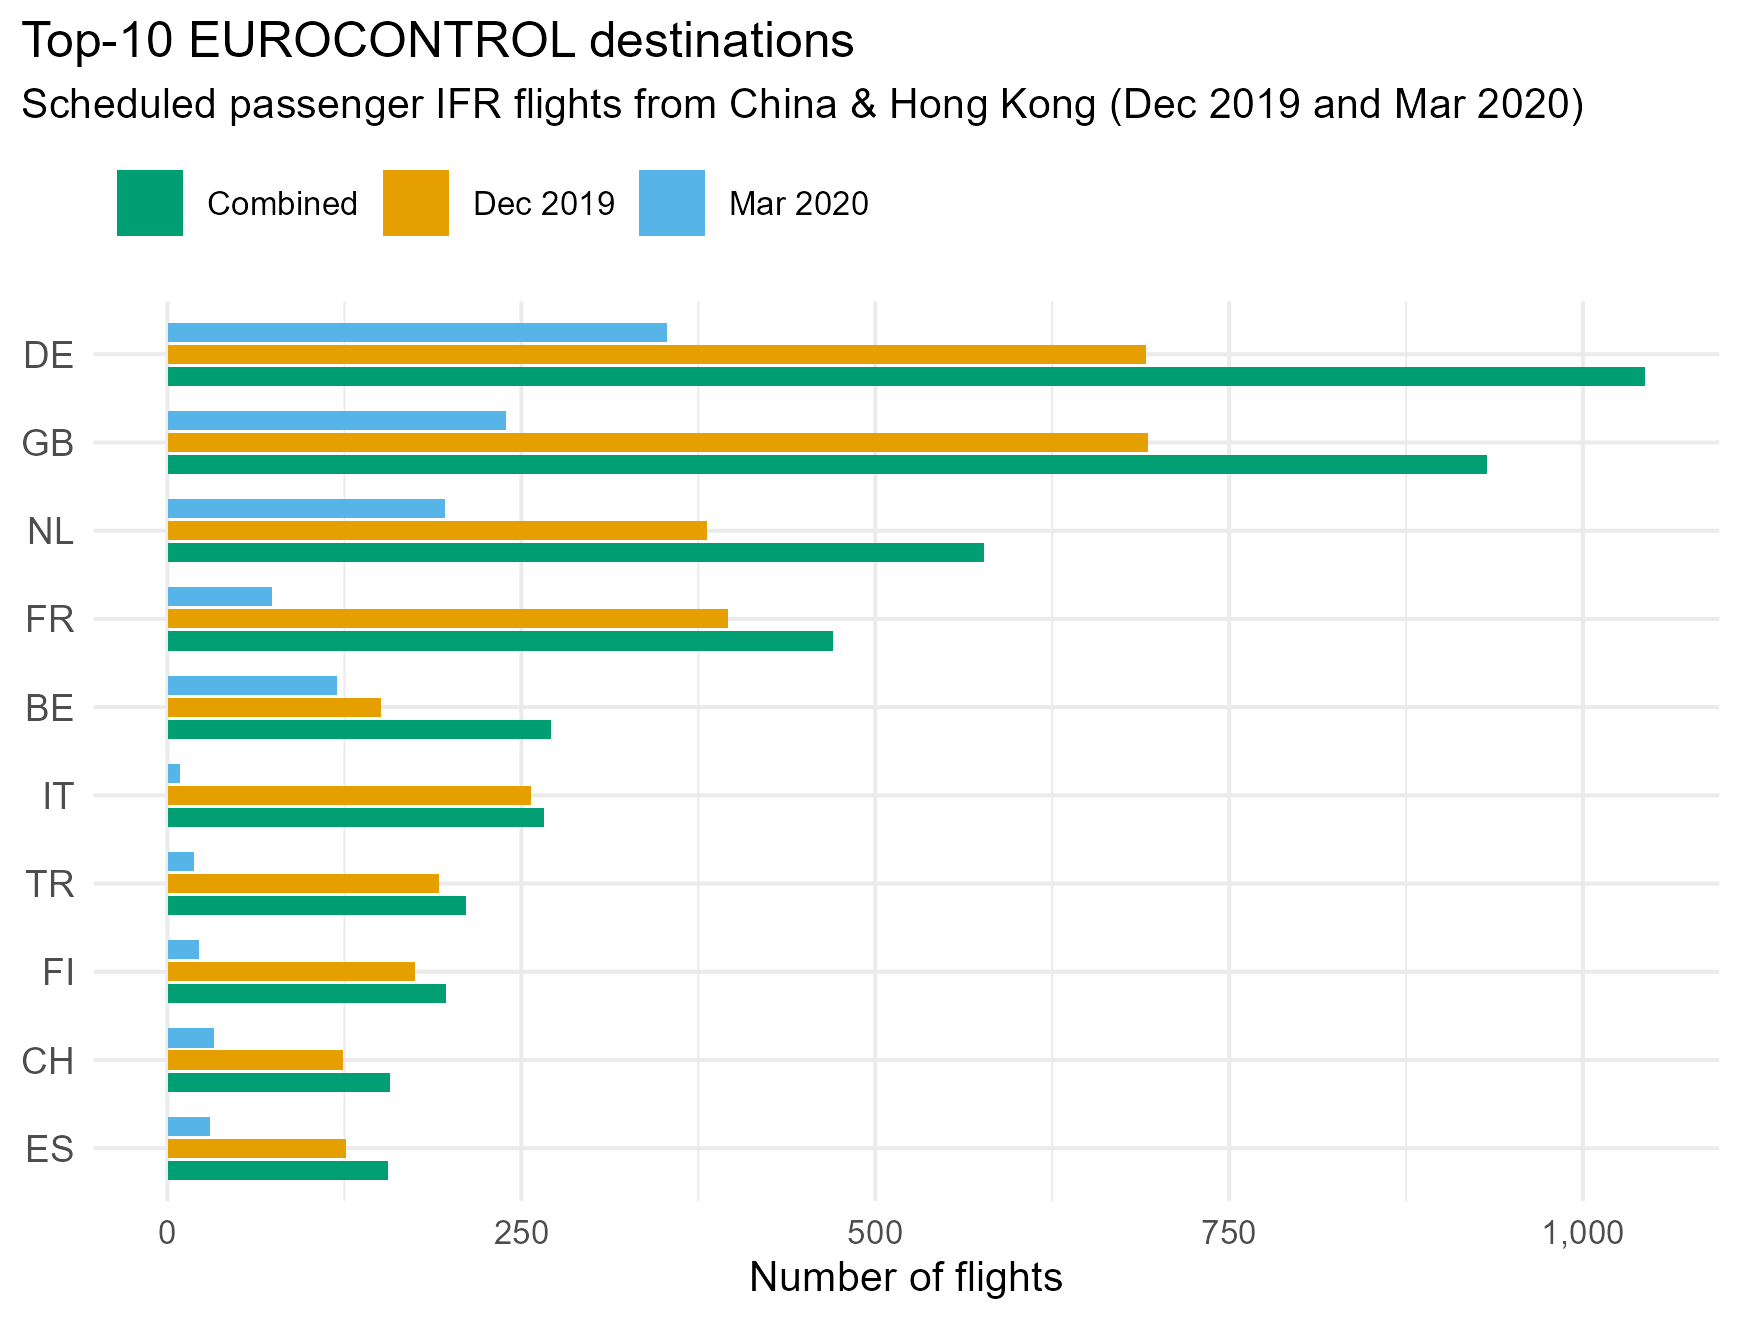
\includegraphics[width=0.8\linewidth,height=\textheight,keepaspectratio]{data/figures/bar_top10_destinations.png}

}

\caption{\label{fig-top10_eu_dest_cntry}Top-10 European destination
countries for direct CN/HK IFR S/N flights in December 2019 (orange),
March 2020 (blue), and combined (green). Bars are counts of filed IFR
scheduled/charter movements (cargo-only F excluded).}

\end{figure}%

\textbf{Take-away.} Import pressure was not evenly distributed: a few
Western gateways carried most movements in both study months, producing
a right-skewed country-level exposure index.

\subsubsection{Route diversity
vs.~volume}\label{route-diversity-vs.-volume}

\phantomsection\label{cell-fig-origins_per_destination}
\begin{figure}[H]

\centering{

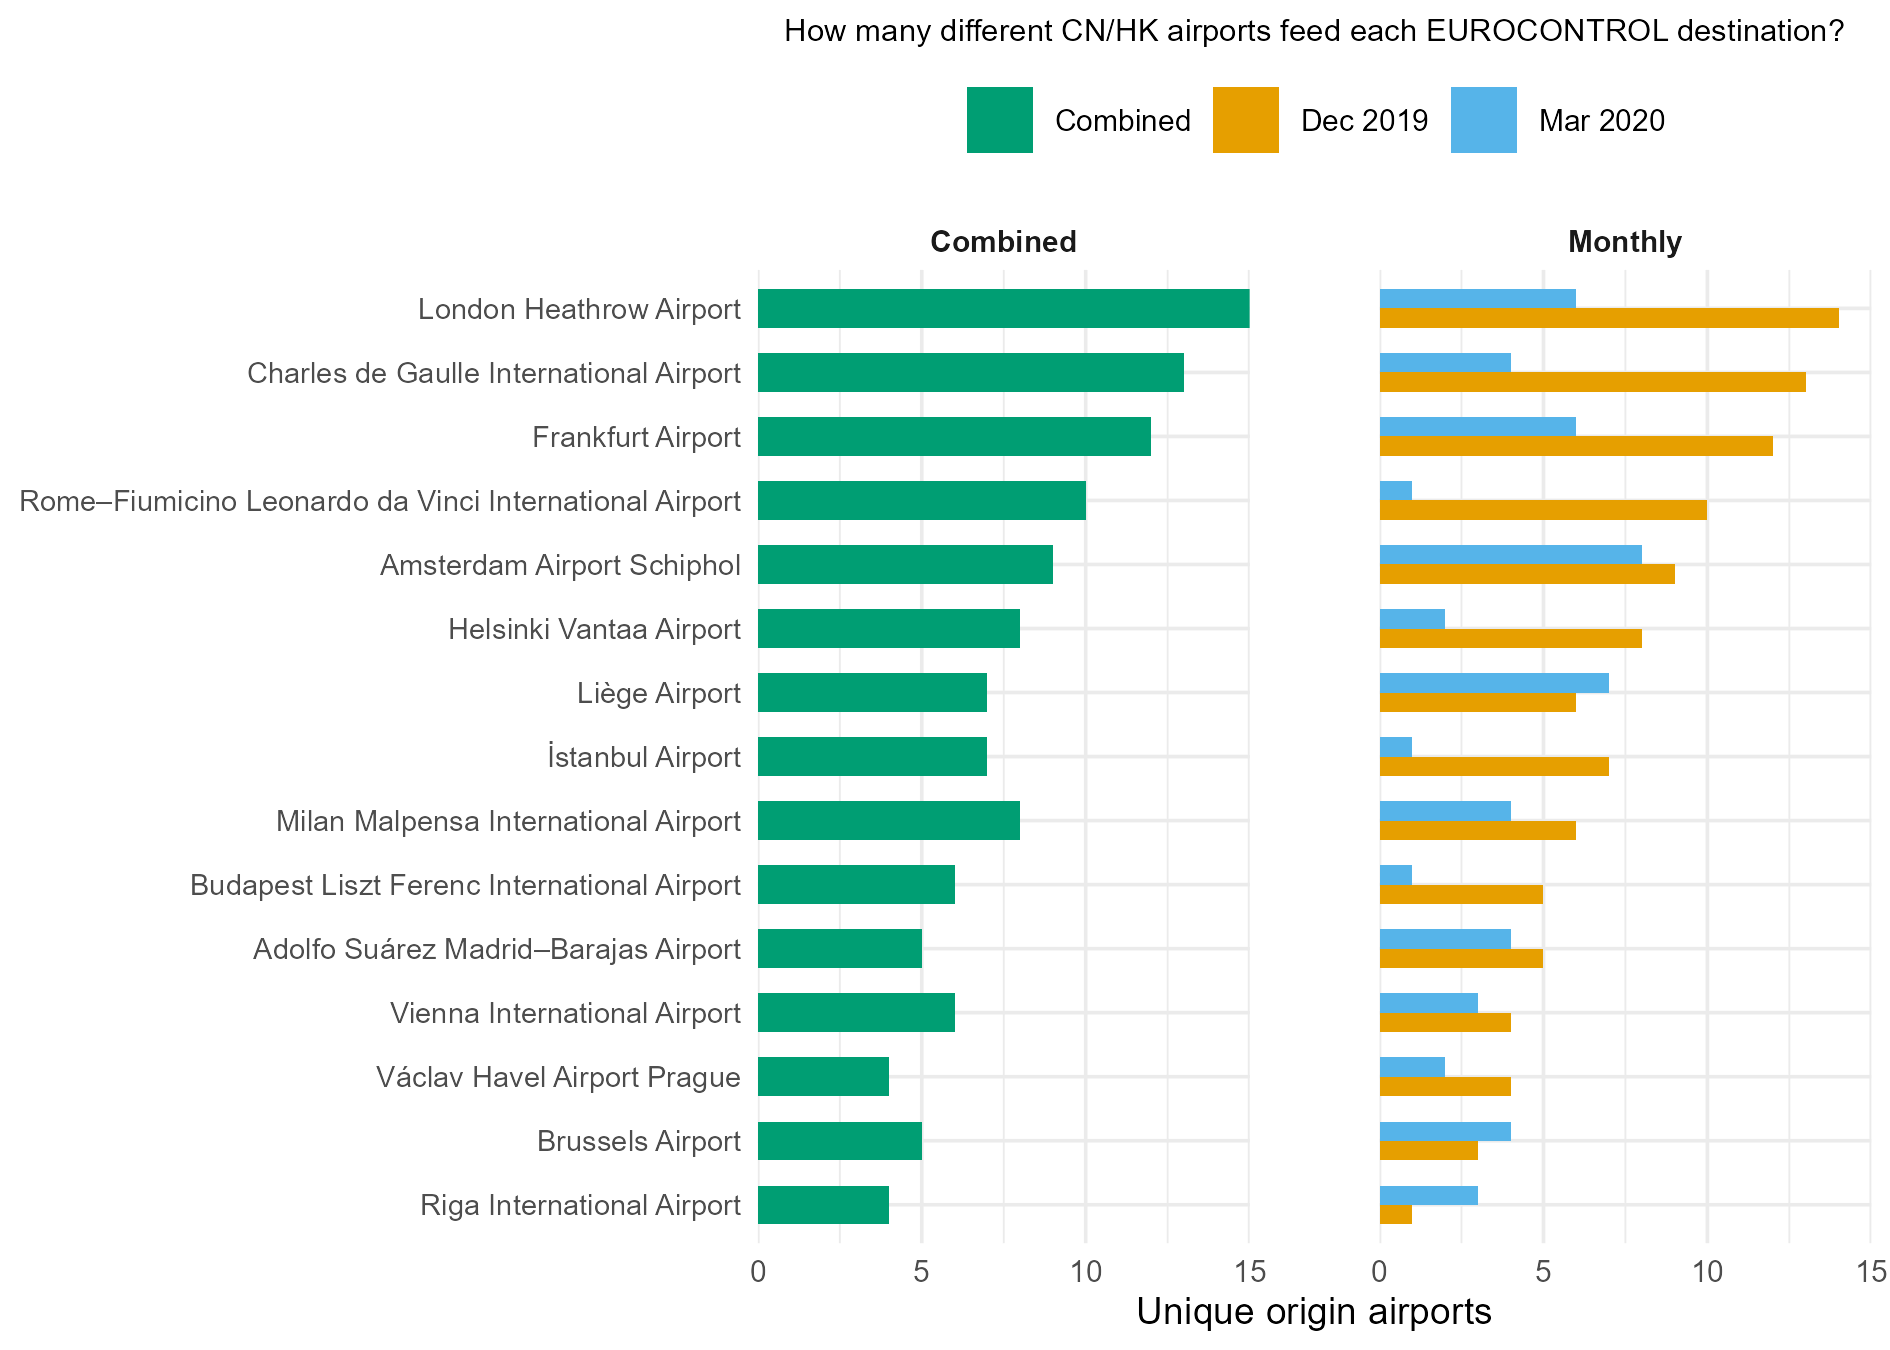
\includegraphics[width=0.8\linewidth,height=\textheight,keepaspectratio]{data/figures/bar_origins_per_destination.png}

}

\caption{\label{fig-origins_per_destination}How many distinct CN/HK
origin airports fed each EUROCONTROL destination? Left: combined
Dec-2019 + Mar-2020; right: month-by-month. Western megahubs
(\textbf{LHR 15}, \textbf{CDG 13}, \textbf{FRA 12}) top the list.
\textbf{Liège (LGG)} ranks high on diversity despite modest volume
because many \textbf{N} flights are cargo charters---illustrating how
movement counts can overstate \textbf{passenger} exposure at
freight-biased airports.}

\end{figure}%

\textbf{Volume and diversity move together.} Each additional
\textasciitilde100 flights is associated with \textbf{1--2} extra
Chinese origin airports (\textbf{ρ ≈ 0.86; \emph{p} \textless{} 0.001;
\emph{n} = 47}).

\phantomsection\label{cell-fig-scatter_volume_vs_origin}
\begin{figure}[H]

\centering{

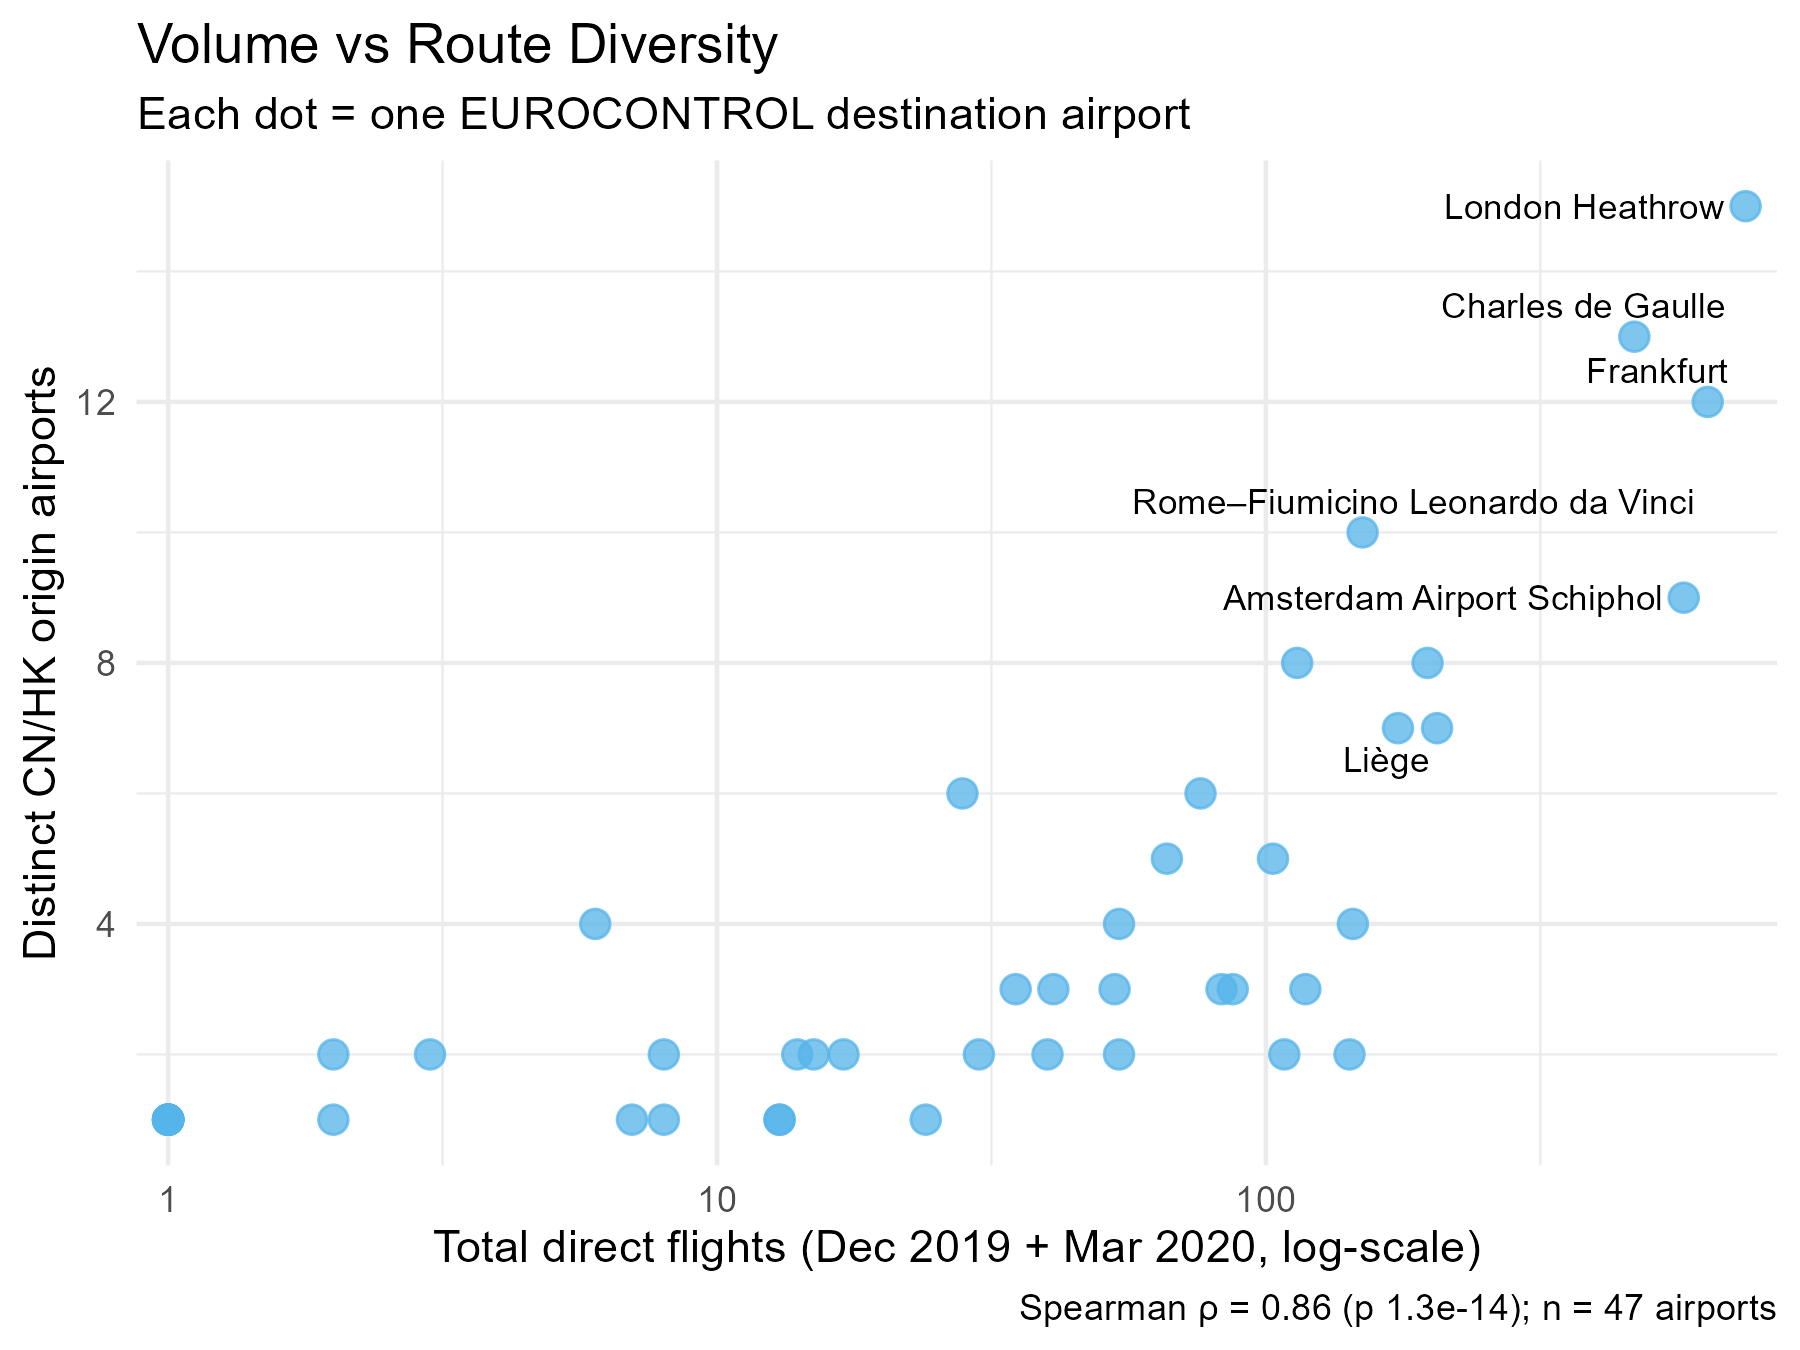
\includegraphics[width=0.8\linewidth,height=\textheight,keepaspectratio]{data/figures/scatter_volume_vs_origins.png}

}

\caption{\label{fig-scatter_volume_vs_origin}Each dot is one destination
airport. X: combined Dec-2019 + Mar-2020 S/N flights (log-scale). Y:
number of distinct CN/HK origin airports. Spearman \(\rho \approx 0.86\)
(\emph{p} \textless{} 0.001; \emph{n} = 47). \textbf{LGG} lies above the
trend---high diversity for moderate volume---because many flights are
cargo charters.}

\end{figure}%

\textbf{Interpretation.} The slope is driven by large passenger hubs in
the upper-right; most other airports remain low-volume/low-diversity.
\textbf{LGG} is freight-biased and inflates ``exposure'' without adding
many travellers (see \hyperref[limitations]{Limitations}).

\subsubsection{March 2020 cliff-edge}\label{march-cliff}

We \textbf{plot only the 21 states} with \textbf{≥ 5} direct CN/HK
flights in Dec-2019 to avoid visually noisy −100\% bars from trivial
baselines (e.g., single charters). The correlation analysis uses the
full \textbf{25-country} panel.

\phantomsection\label{cell-fig-pct_change_filtered}
\begin{figure}[H]

\centering{

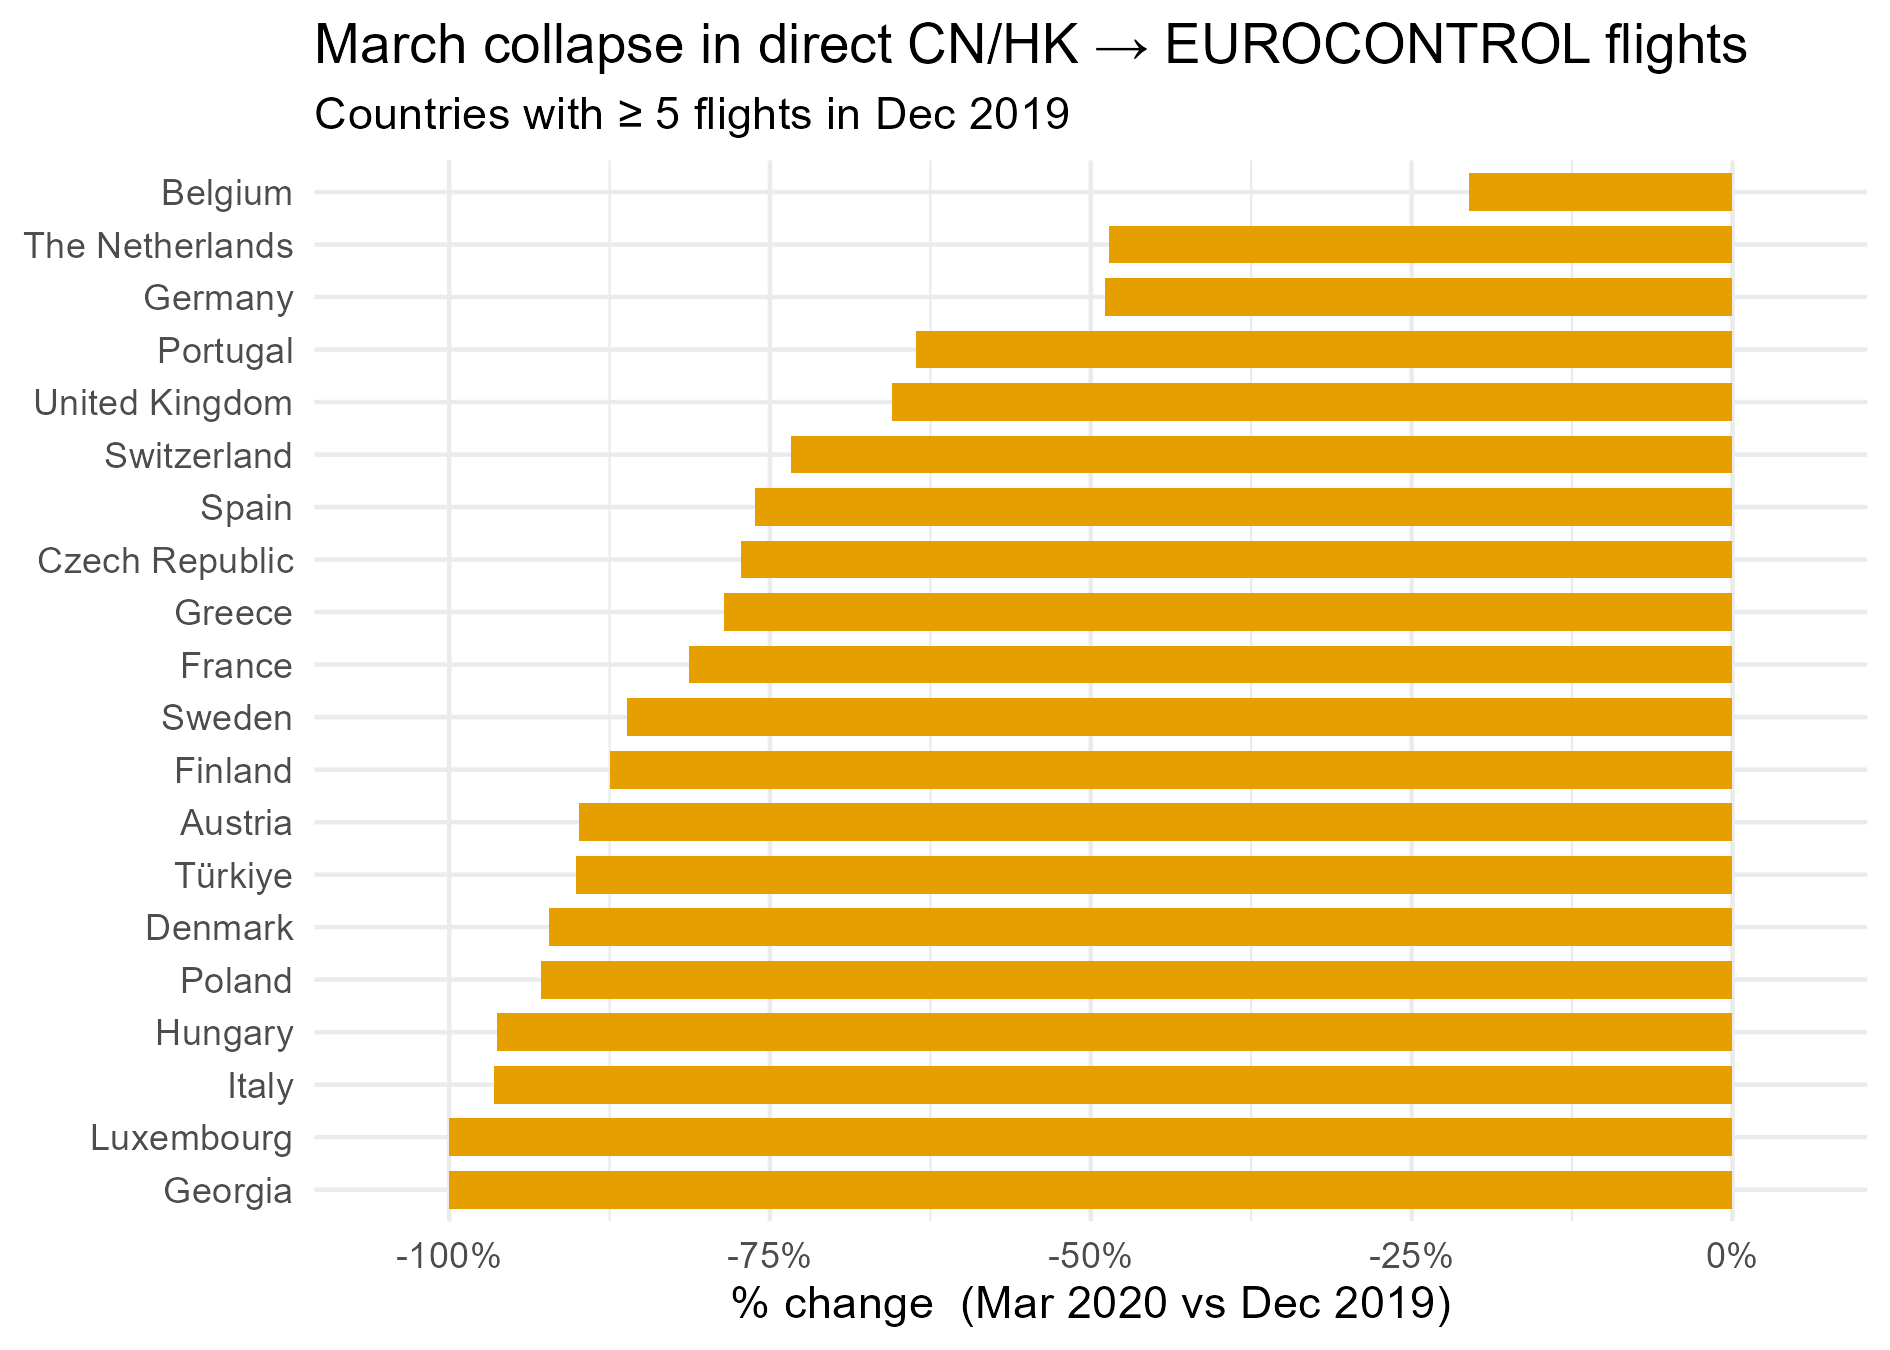
\includegraphics[width=0.8\linewidth,height=\textheight,keepaspectratio]{data/figures/pct_change_filtered.png}

}

\caption{\label{fig-pct_change_filtered}Percentage change in direct
CN/HK S/N flights from Dec-2019 baseline to Mar-2020 for countries with
≥5 December flights (\emph{n} = 21). All countries cut traffic by at
least 50\%; 7/21 reduced \textgreater90\%, and 14/21 ≥75\%. The
Netherlands and Germany retained the largest residual shares; most
others were near zero.}

\end{figure}%

\textbf{What the figure shows.} Among the \textbf{21 ≥ 5-flight
countries}, every one cut traffic by \textbf{≥ 50\%} by late March 2020:

\begin{itemize}
\tightlist
\item
  \textbf{7 of 21} slashed \textbf{\textgreater{} 90\%} (bars pinned
  near −100\%).
\item
  \textbf{14 of 21} cut \textbf{≥ 75\%} --- a tightly synchronised
  shutdown.
\item
  \textbf{The Netherlands and Germany} retained the largest
  \textbf{percentage} shares; several others, including
  \textbf{Belgium}, retained \textbf{lower percentage shares} but can
  still rank high in \textbf{absolute} counts.
\end{itemize}

\begin{longtable}[]{@{}
  >{\raggedright\arraybackslash}p{(\linewidth - 2\tabcolsep) * \real{0.2200}}
  >{\raggedright\arraybackslash}p{(\linewidth - 2\tabcolsep) * \real{0.7800}}@{}}
\caption{Signals at the March-2020 cliff-edge and their implications for
analysis.}\label{tbl-cliff-signals}\tabularnewline
\toprule\noalign{}
\begin{minipage}[b]{\linewidth}\raggedright
Signal
\end{minipage} & \begin{minipage}[b]{\linewidth}\raggedright
Take-away
\end{minipage} \\
\midrule\noalign{}
\endfirsthead
\toprule\noalign{}
\begin{minipage}[b]{\linewidth}\raggedright
Signal
\end{minipage} & \begin{minipage}[b]{\linewidth}\raggedright
Take-away
\end{minipage} \\
\midrule\noalign{}
\endhead
\bottomrule\noalign{}
\endlastfoot
\textbf{Timing} & The plunge aligns with EU actions restricting
\textbf{non-essential travel to the EU} (Commission Communication,
\textbf{16 Mar 2020}; later codified by \textbf{Council Recommendation
(EU) 2020/912}, \textbf{30 Jun 2020}) and the CAAC \textbf{``Five-One''}
policy (\textbf{26 Mar 2020}) limiting international passenger services
to \textbf{one route per airline per country} with \textbf{at most one
weekly flight}.
\citep{eu-comm-2020-travel, eu-council-2020-912, CAAC2020} \\
\textbf{Uniformity} & Because the contraction is pan-European, any
exposure--mortality link must be driven by traffic that occurred
\textbf{before} the cliff. \\
\textbf{Residual risk} & Absolute counts still diverged after March: a
few hubs kept \textbf{\textasciitilde200--350} rotations, so a trickle
of import potential remained (see Δ-flights in
Table~\ref{tbl-collapse}). \\
\end{longtable}

\textbf{Data note (capacity vs movements).} The OAG figures cited
elsewhere report \textbf{scheduled passenger seat capacity} only;
\textbf{charter} operations and \textbf{all-cargo} flights are excluded.
Accordingly, these series should be \textbf{interpreted as a capacity
baseline}, not as counts of movements or passengers.
\citep{warnocksmith2021}

With direct CN/HK traffic reduced to a trickle after late March, any
variation in \textbf{first-wave} excess mortality must trace back to
flights that arrived \textbf{before} the cliff-edge. The next subsection
tests whether pre-collapse exposure leaves a statistical imprint in the
\textbf{5 May 2020} snapshot.

\subsection{Association with first-wave mortality}\label{baseline-2020}

\begin{longtable}[]{@{}lrrrrlr@{}}

\caption{\label{tbl-spearman_2020}Spearman \(\rho\) between early
flight-exposure metrics and excess mortality on 5 May 2020 (95\%
bootstrap CI; n = 25). Significant results (\emph{p} \textless{} 0.05)
marked ✓.}

\tabularnewline

\toprule\noalign{}
variable & rho & ci\_lo & ci\_hi & p & sig & n \\
\midrule\noalign{}
\endhead
\bottomrule\noalign{}
\endlastfoot
Dec 2019 & 0.502 & 0.135 & 0.759 & 0.011 & ✓ & 25 \\
Mar 2020 & 0.573 & 0.228 & 0.796 & 0.003 & ✓ & 25 \\
Combined & 0.526 & 0.177 & 0.771 & 0.007 & ✓ & 25 \\
Flights / M pop & 0.303 & -0.077 & 0.606 & 0.141 & --- & 25 \\

\end{longtable}

\textbf{Reading the 2020 snapshot.} All four exposure metrics are
\textbf{positively} associated with first-wave excess mortality
(Table~\ref{tbl-spearman_2020}). Three are statistically significant;
the population-scaled metric is positive but not significant. Using the
\textbf{Dec + Mar combined} count:

\begin{itemize}
\tightlist
\item
  Spearman \(\rho = 0.526\) (95\% CI \textbf{0.177--0.771}, \emph{p} =
  0.007; \emph{n} = 25).
\item
  Countries in the \textbf{top exposure quartile} recorded \textbf{≈ 465
  excess deaths / million} more than those in the bottom quartile
  (median gap).
\item
  Figure~\ref{fig-scatter-2020} shows an overall positive slope with
  \textbf{notable vertical outliers} (e.g., \textbf{ESP} with high
  mortality despite fewer direct flights; \textbf{DEU} with lower
  mortality given its volume).
\end{itemize}

\phantomsection\label{cell-fig-scatter-2020}
\begin{figure}[H]

\centering{

\pandocbounded{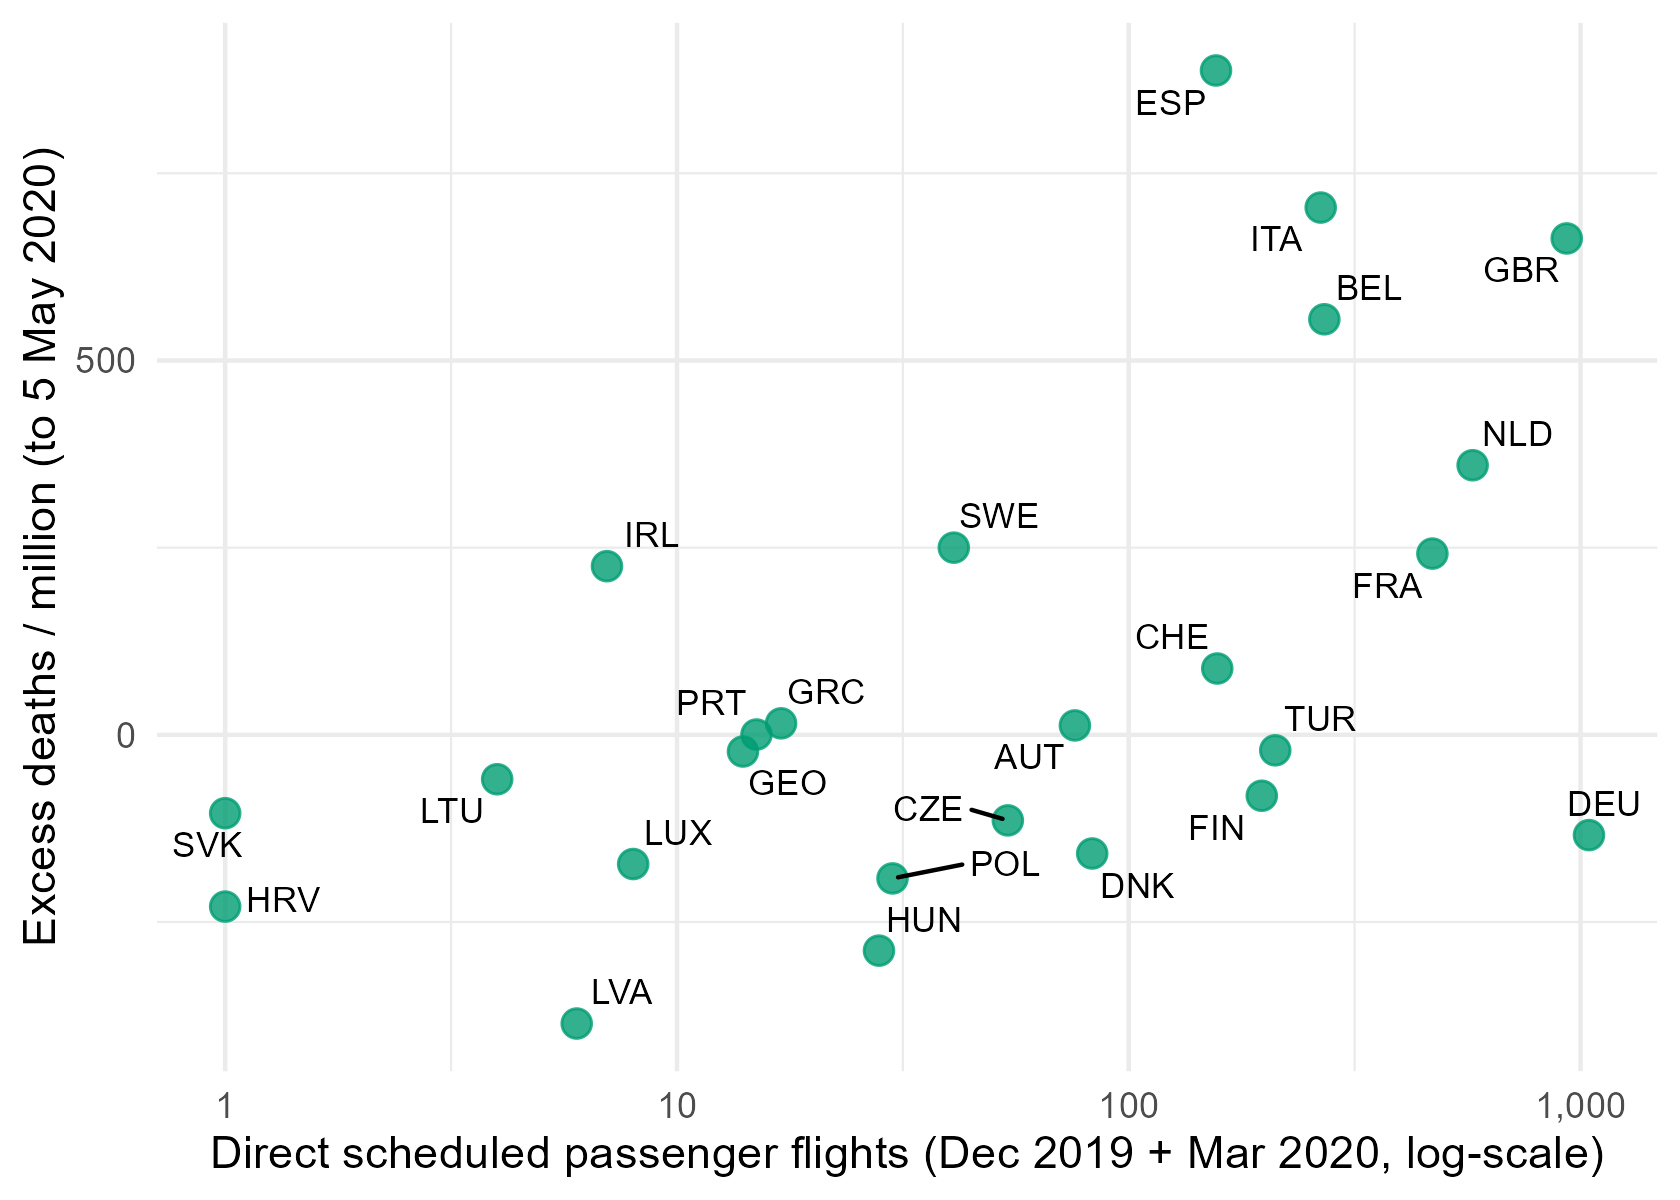
\includegraphics[keepaspectratio]{data/figures/scatter_2020.png}}

}

\caption{\label{fig-scatter-2020}Direct CN/HK S/N flights (Dec-2019 +
Mar-2020, log-scale) versus excess deaths per million on 5 May 2020 (n =
25). Spearman \(\rho \approx 0.53\) (\emph{p} \textless{} 0.01). Several
Western hubs anchor the right tail; \textbf{ESP} is a high-mortality
outlier at moderate exposure.}

\end{figure}%

\subsection{Evolution 2021--2023}\label{evolution-2021-2023}

\phantomsection\label{cell-fig-rho_caterpillar}
\begin{figure}[H]

\centering{

\pandocbounded{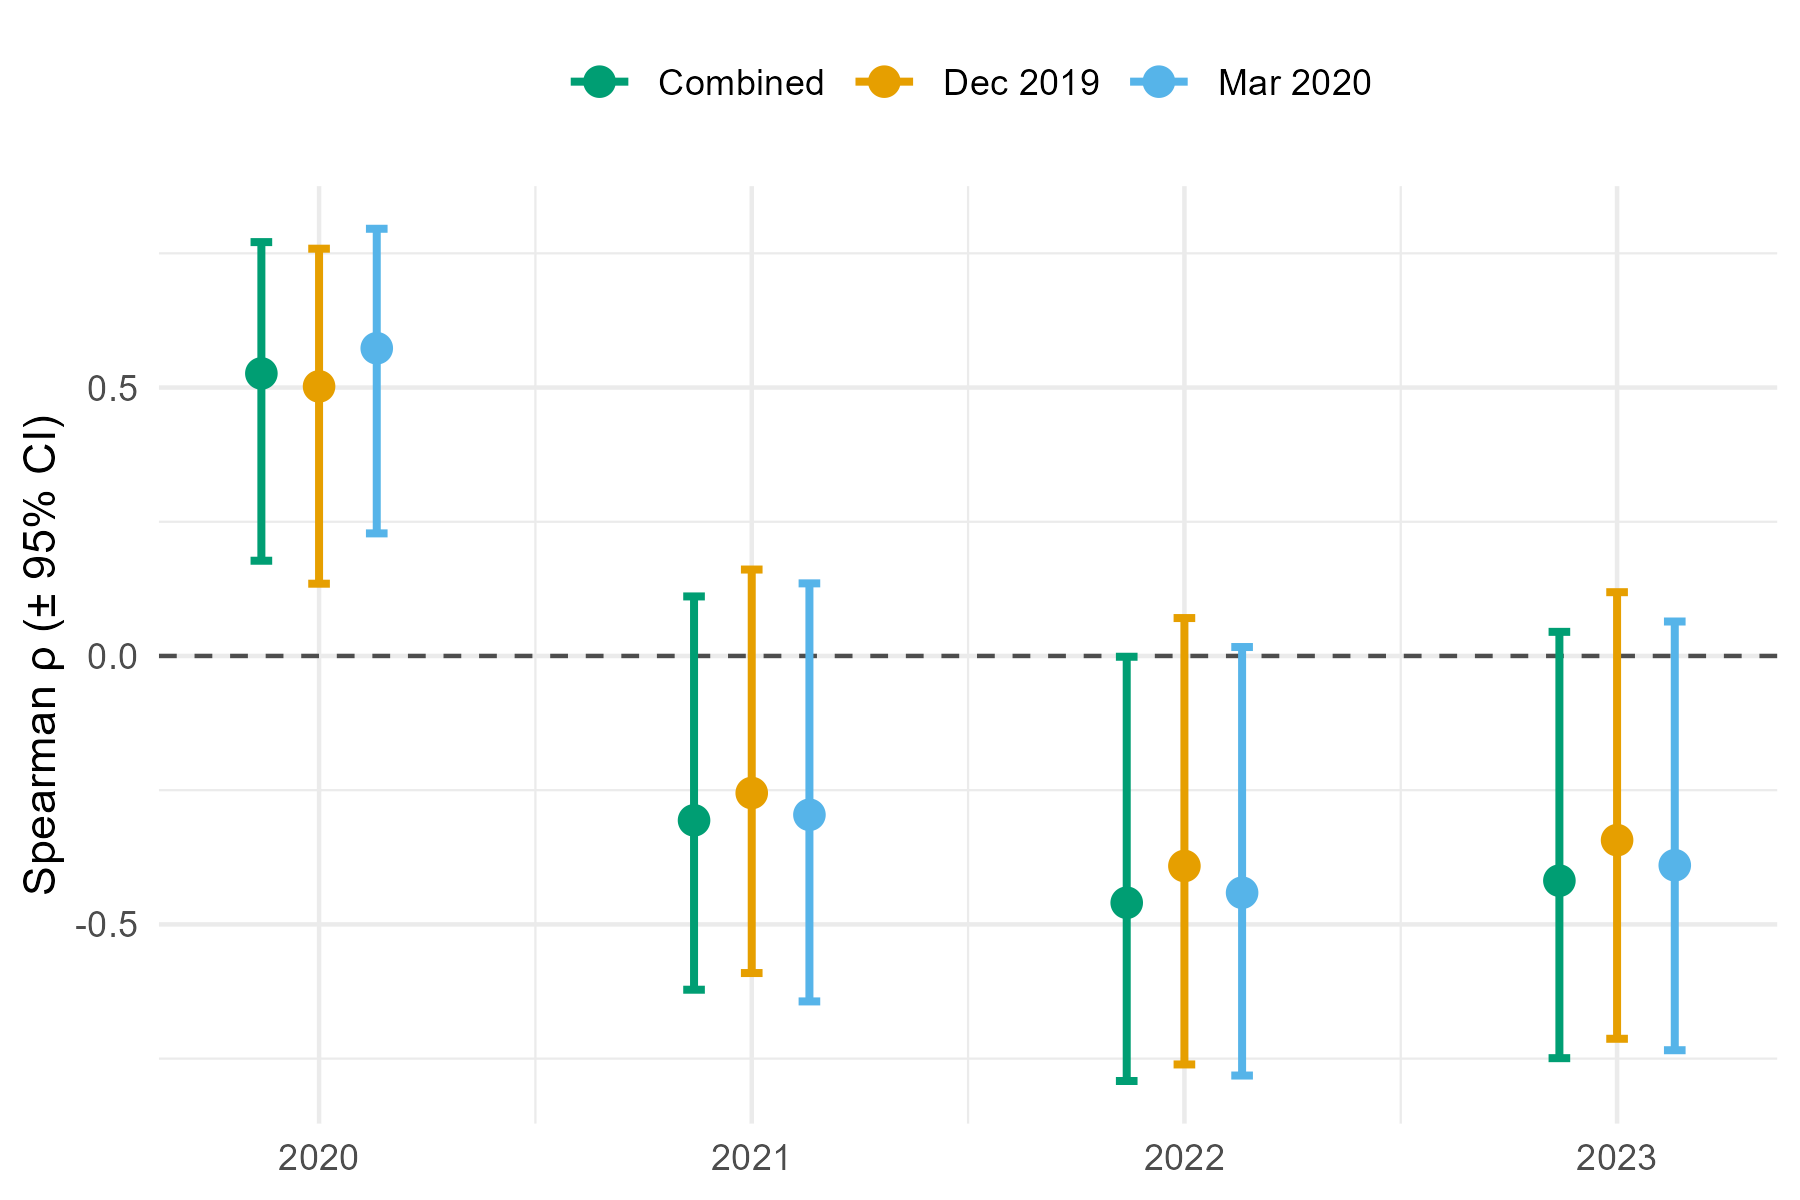
\includegraphics[keepaspectratio]{data/figures/rho_caterpillar.png}}

}

\caption{\label{fig-rho_caterpillar}Spearman \(\rho\) (points) with 95\%
bootstrap CIs (bars) for Dec-2019, Mar-2020, and their sum. Estimates
are positive in 2020. From 2021 onward they trend toward zero or below;
in 2022 the Mar and Combined metrics are significantly negative. In 2023
they remain negative with CIs that touch or narrowly include zero.}

\end{figure}%

\textbf{Pattern.} Estimates are \textbf{positive} in 2020, weaken toward
\textbf{zero} in 2021, and turn \textbf{negative} in 2022--2023. For the
\textbf{Combined} metric:

\begin{itemize}
\tightlist
\item
  \textbf{2020:} \textbf{ρ = 0.526} (95\% CI 0.177--0.771; \emph{p} =
  0.007)
\item
  \textbf{2021:} \textbf{ρ = −0.306} (95\% CI −0.622--0.111; n.s.)
\item
  \textbf{2022:} \textbf{ρ = −0.460} (95\% CI −0.792 to −0.001; \emph{p}
  ≈ 0.02)
\item
  \textbf{2023:} \textbf{ρ = −0.419} (95\% CI −0.749--0.045;
  \textbf{borderline}; CI grazes zero)
\end{itemize}

\begin{longtable}[]{@{}rrrr@{}}

\caption{\label{tbl-sensitivity}Sensitivity: baseline vs partial
Spearman controlling for population ≥ 65 y.}

\tabularnewline

\toprule\noalign{}
year & ρ baseline & ρ adj age 65+ & p adj \\
\midrule\noalign{}
\endhead
\bottomrule\noalign{}
\endlastfoot
2020 & 0.526 & 0.525 & 0.008 \\
2021 & -0.306 & -0.289 & 0.171 \\
2022 & -0.460 & -0.456 & 0.025 \\
2023 & -0.419 & -0.424 & 0.039 \\

\end{longtable}

\textbf{Sensitivity \& partial checks.} Adjusting for the share aged ≥
65 leaves effect sizes essentially unchanged
(\textbf{\textbar Δρ\textbar{} ≤ 0.02}) and does not alter any year's
inference; age structure cannot explain the sign flip.

\paragraph{Vaccination coverage by exposure quartile (May
2022)}\label{vaccination-coverage-by-exposure-quartile-may-2022}

\begin{longtable}[]{@{}lll@{}}

\caption{\label{tbl-vaccination_exposure_res}Full-vaccination coverage
on 5 May 2022 (±7 days) by flight-exposure quartile (baseline = Dec-2019
+ Mar-2020 flights; OWID
\texttt{people\_fully\_vaccinated\_per\_hundred}).}

\tabularnewline

\toprule\noalign{}
Exposure quartile & Median full-vax \% & n \\
\midrule\noalign{}
\endhead
\bottomrule\noalign{}
\endlastfoot
Q1 & 69.3 \% & n = 7 \\
Q2 & 65.5 \% & n = 6 \\
Q3 & 62.1 \% & n = 6 \\
Q4 & 78.0 \% & n = 6 \\

\end{longtable}

\textbf{Gradient.} Median full-vaccination rises from \textbf{Q3 ≈ 62\%}
and \textbf{Q1 ≈ 69\%} to \textbf{Q4 ≈ 78\%} (\emph{n} per quartile in
table), consistent with wealth/governance gradients and the
weakening/negative \(\rho\) in 2021--2023.

\subsection{Results summary}\label{results-summary}

\begin{itemize}
\tightlist
\item
  \textbf{2020:} heavier direct CN/HK exposure ↔ \textbf{higher}
  first-wave excess mortality (\textbf{ρ ≈ 0.53}).
\item
  \textbf{2021:} association ≈ \textbf{zero}.
\item
  \textbf{2022--2023:} association \textbf{negative} (significant in
  \textbf{2022}; \textbf{negative/borderline} in \textbf{2023}).
\item
  \textbf{Population-scaled exposure} flips \textbf{earlier} (negative
  by \textbf{2021}).
\end{itemize}

\section{Discussion}\label{discussion}

\subsection{Interpreting the reversal
(2021--2023)}\label{interpreting-the-reversal-20212023}

\begin{itemize}
\item
  \textbf{Wealth \& structural vulnerability.} Excess mortality tends to
  \textbf{fall with GDP per capita} and \textbf{rise with
  poverty/inequality}, which helps explain why the positive
  flight--mortality link \textbf{vanishes after 2020}: Europe's most
  connected hubs (Germany, the UK, the Netherlands, France) also sit in
  the top-GDP tercile and had more protective structural factors.
  \citep{ioannidis2023}
\item
  \textbf{Vaccination rollout.} By \textbf{5 May 2022} (±7 days), the
  \textbf{highest-exposure quartile (Q4)} had \textbf{higher
  full-vaccination} than lower-exposure quartiles (see
  Table~\ref{tbl-vaccination_exposure_res}), aligning with OWID's series
  and helping explain the \textbf{post-2020 attenuation/flip}.
  \citep{mathieu2021owidvaccinations}
\item
  \textbf{Policy timing \& capacity.} Comparative work shows
  \textbf{travel curbs mostly delay} spread unless paired with local
  measures. \citep{chinazzi2020} In Europe, the \textbf{slot-waiver}
  adopted in late March 2020 \textbf{removed the 80/20
  ``use-it-or-lose-it'' incentive}, coinciding with a \textbf{drop in
  statistically abnormal low-load flights} documented for EU carriers.
  \citep{sun2022_a, sun2022_b} Together with vaccination and
  governance-capacity gradients \citep{rahmanian2024}, this helps
  rationalise the \textbf{2022--2023 sign-flip}.
\end{itemize}

\subsection{Strengths}\label{strengths}

\begin{itemize}
\tightlist
\item
  \textbf{Regulator-grade exposure.} \textbf{ADRR} captures
  \textbf{every filed IFR passenger movement touching European
  airspace}, avoiding known East Asia \textbf{ADS-B gaps} and
  origin/destination ambiguities. \citep{strohmeier2021}
\item
  \textbf{Lean, transparent cleaning.} \textbf{S/N} only; exact re-files
  de-duplicated; scripts and derived tables alongside the manuscript.
  \citep{eurocontrol2022seg}
\item
  \textbf{Reproducibility.} End-to-end R + Quarto with \texttt{build.sh}
  and \texttt{renv.lock}; \textbf{5,000-draw bootstrap CIs} for every
  Spearman \(\rho\).
\end{itemize}

\subsection{Limitations}\label{limitations}

\begin{itemize}
\tightlist
\item
  \textbf{Load-factor bias.} Many EU carriers operated
  \textbf{statistically ``abnormal'' low-load} flights in
  \textbf{Mar--Apr 2020}, with shares receding through 2021;
  ``abnormal'' is defined \textbf{statistically} (IQR outliers vs
  2017--2019 baselines), \textbf{not} by a fixed occupancy cut-off
  (e.g., \emph{under 10\% of seats filled}). Hence \(F_{\text{SUM}}\)
  measures \textbf{potential seeding capacity}, not realised traveller
  volumes. \citep{sun2022_b} At a major hub like \textbf{Frankfurt},
  passenger volumes collapsed while cargo shifted to freighters and
  ``preighters.'' \citep{fraport2021}
\item
  \textbf{February gap.} No public \textbf{ADRR} slice for \textbf{Feb
  2020} → peak early-exposure may be \textbf{under-estimated}.
\item
  \textbf{Indirect legs invisible.} Multi-leg routings (e.g.,
  \textbf{PVG → DXB → VIE}) and non-air links aren't captured.
\item
  \textbf{Ecological, small \emph{n}.} A country-level panel
  (\textasciitilde25 units) can't resolve within-state heterogeneity;
  residual confounding remains possible.
\end{itemize}

\subsection{Methodological
reflections}\label{methodological-reflections}

The project was \textbf{initially envisioned} as a global
effective-distance SIR exercise \citep{brockmann2013}, but we did not
proceed beyond scoping. Two constraints drove an early pivot: (i) sparse
\textbf{East Asia ADS-B coverage} (and OpenSky's flight-derivation
quirks) \citep{strohmeier2021}, and (ii) no \textbf{February} ADRR
snapshot (public months are \textbf{Mar \textbar{} Jun \textbar{} Sep
\textbar{} Dec}). Given those constraints---and a BA time-box---we
adopted an exploratory, fully reproducible \textbf{rank-correlation}
design on \textbf{Dec 2019} and \textbf{Mar 2020} exposures against
\textbf{four} annual excess-mortality snapshots.

\subsection{Implications \& directions for future
research}\label{implications-directions-for-future-research}

\textbf{What the results do say.} Direct CN/HK flight volumes help
explain cross-country differences in \textbf{spring 2020} excess
mortality.

\textbf{What they don't say.} Ecological, rank-based associations do
\textbf{not} identify causal effects or passenger-level transmission.

\textbf{Future work (beyond the scope of this study).}

\begin{enumerate}
\def\labelenumi{\arabic{enumi}.}
\tightlist
\item
  \textbf{Passenger weighting.} Combine ADRR movements with IATA/OAG
  load factors to down-weight ``ghost flights'' and approximate imported
  passenger volumes.
\item
  \textbf{Multi-leg \& multimodal import paths.} Reconstruct OD chains
  (air--air and air--land/sea) to capture indirect routes (e.g., PVG →
  DXB → VIE) and non-air entries.
\item
  \textbf{Sub-national resolution.} Build NUTS-2 or airport-catchment
  panels to reduce ecological bias and align exposure with local
  mortality.
\item
  \textbf{Integrated transmission models.} Embed exposure in network
  SEIR/SEnIR frameworks with NPIs, vaccination, and health-system
  capacity to move from association to mechanism.
\end{enumerate}

\subsection{Conclusion}\label{conclusion}

\textbf{Flight counts} are a useful proxy for \textbf{initial import
pressure}: they \textbf{correlate with first-wave excess mortality} but
\textbf{not} with later outcomes, which align more with
\textbf{vaccination}, \textbf{policy timing}, and \textbf{system
capacity}.

\section{References}\label{references}

\renewcommand{\bibsection}{}
\bibliography{thesis_ref.bib}

\section{Acknowledgments}\label{acknowledgments}

\emph{This thesis uses the Aviation Data Repository for Research (ADRR)
made available by EUROCONTROL © 2025. EUROCONTROL does not necessarily
endorse the conclusions and shall not be liable for any direct,
indirect, incidental or consequential damages arising out of or in
connection with this work.}

I would also like to thank my supervisor, Christian Neuwirth, for his
trust, which allowed me to refine my skills and learn a great deal over
the past years --- with the guidance of a mentor, even if unofficial.

\section{Appendix}\label{appendix}

\subsection{Supplementary methods \& figures}\label{appendix-a}

\subsubsection{Coverage audit --- EUROCONTROL vs
OpenSky}\label{coverage-audit-eurocontrol-vs-opensky}

OpenSky's community ADS-B coverage in early 2020 is
uneven---\textbf{strong in Western Europe}, \textbf{thin over East Asia}
and parts of \textbf{Eastern Europe} so it \textbf{undercounts} direct
CN/HK arrivals relative to EUROCONTROL ADRR. In our audit, OpenSky
\textbf{misses} five countries entirely and \textbf{undercounts} most
others; we therefore treat OpenSky as a \textbf{QC benchmark only}.
\citep{strohmeier2021}

\begin{longtable}[]{@{}
  >{\raggedright\arraybackslash}p{(\linewidth - 14\tabcolsep) * \real{0.0549}}
  >{\raggedleft\arraybackslash}p{(\linewidth - 14\tabcolsep) * \real{0.1538}}
  >{\raggedleft\arraybackslash}p{(\linewidth - 14\tabcolsep) * \real{0.1538}}
  >{\raggedleft\arraybackslash}p{(\linewidth - 14\tabcolsep) * \real{0.1538}}
  >{\raggedleft\arraybackslash}p{(\linewidth - 14\tabcolsep) * \real{0.1538}}
  >{\raggedleft\arraybackslash}p{(\linewidth - 14\tabcolsep) * \real{0.1538}}
  >{\raggedright\arraybackslash}p{(\linewidth - 14\tabcolsep) * \real{0.0879}}
  >{\raggedright\arraybackslash}p{(\linewidth - 14\tabcolsep) * \real{0.0879}}@{}}

\caption{\label{tbl-os-vs-eu-full}Direct CN/HK arrivals captured by
EUROCONTROL ADRR (EU) vs OpenSky (OS). Rows sorted by ADRR Dec-2019
counts. OS reflects receiver coverage, not filed IFR (S/N passenger
traffic only).}

\tabularnewline

\toprule\noalign{}
\begin{minipage}[b]{\linewidth}\raggedright
iso3
\end{minipage} & \begin{minipage}[b]{\linewidth}\raggedleft
Dec 2019 (EU)
\end{minipage} & \begin{minipage}[b]{\linewidth}\raggedleft
Mar 2020 (EU)
\end{minipage} & \begin{minipage}[b]{\linewidth}\raggedleft
Dec 2019 (OS)
\end{minipage} & \begin{minipage}[b]{\linewidth}\raggedleft
Feb 2020 (OS)
\end{minipage} & \begin{minipage}[b]{\linewidth}\raggedleft
Mar 2020 (OS)
\end{minipage} & \begin{minipage}[b]{\linewidth}\raggedright
EU\_only
\end{minipage} & \begin{minipage}[b]{\linewidth}\raggedright
OS\_only
\end{minipage} \\
\midrule\noalign{}
\endhead
\bottomrule\noalign{}
\endlastfoot
GBR & 693 & 239 & 299 & 227 & 145 & FALSE & FALSE \\
DEU & 691 & 353 & 174 & 123 & 153 & FALSE & FALSE \\
FRA & 396 & 74 & 63 & 53 & 21 & FALSE & FALSE \\
NLD & 381 & 196 & 72 & 60 & 34 & FALSE & FALSE \\
ITA & 257 & 9 & 61 & 1 & 2 & FALSE & FALSE \\
TUR & 192 & 19 & 3 & 0 & 4 & FALSE & FALSE \\
FIN & 175 & 22 & 60 & 47 & 22 & FALSE & FALSE \\
BEL & 151 & 120 & 58 & 38 & 46 & FALSE & FALSE \\
ESP & 126 & 30 & 43 & 27 & 7 & FALSE & FALSE \\
CHE & 124 & 33 & 60 & 54 & 35 & FALSE & FALSE \\
DNK & 77 & 6 & 15 & 18 & 4 & FALSE & FALSE \\
AUT & 69 & 7 & 16 & 6 & 10 & FALSE & FALSE \\
CZE & 44 & 10 & 9 & 0 & 3 & FALSE & FALSE \\
SWE & 36 & 5 & 3 & 2 & 0 & FALSE & FALSE \\
POL & 28 & 2 & 1 & 1 & 0 & FALSE & FALSE \\
HUN & 27 & 1 & 9 & 5 & 10 & FALSE & FALSE \\
GEO & 14 & 0 & 0 & 0 & 0 & TRUE & FALSE \\
GRC & 14 & 3 & 2 & 0 & 1 & FALSE & FALSE \\
PRT & 11 & 4 & 0 & 0 & 0 & TRUE & FALSE \\
LUX & 8 & 0 & 25 & 6 & 37 & FALSE & FALSE \\
UKR & 6 & 2 & 0 & 0 & 0 & TRUE & FALSE \\
LTU & 1 & 3 & 0 & 0 & 1 & FALSE & FALSE \\
LVA & 1 & 5 & 0 & 5 & 4 & FALSE & FALSE \\
ALB & 0 & 0 & 0 & 0 & 0 & FALSE & FALSE \\
ARM & 0 & 0 & 0 & 0 & 0 & FALSE & FALSE \\
BGR & 0 & 0 & 0 & 0 & 0 & FALSE & FALSE \\
BIH & 0 & 0 & 0 & 0 & 0 & FALSE & FALSE \\
CYP & 0 & 0 & 0 & 0 & 0 & FALSE & FALSE \\
EST & 0 & 0 & 0 & 0 & 0 & FALSE & FALSE \\
HRV & 0 & 1 & 0 & 0 & 0 & TRUE & FALSE \\
IRL & 0 & 7 & 0 & 1 & 0 & FALSE & FALSE \\
MCO & 0 & 0 & 0 & 0 & 0 & FALSE & FALSE \\
MDA & 0 & 0 & 0 & 0 & 0 & FALSE & FALSE \\
MKD & 0 & 0 & 0 & 0 & 0 & FALSE & FALSE \\
MLT & 0 & 0 & 0 & 0 & 0 & FALSE & FALSE \\
MNE & 0 & 0 & 0 & 0 & 0 & FALSE & FALSE \\
NOR & 0 & 0 & 0 & 0 & 0 & FALSE & FALSE \\
ROU & 0 & 0 & 0 & 0 & 0 & FALSE & FALSE \\
SRB & 0 & 0 & 0 & 0 & 0 & FALSE & FALSE \\
SVK & 0 & 1 & 0 & 0 & 0 & TRUE & FALSE \\
SVN & 0 & 0 & 0 & 0 & 0 & FALSE & FALSE \\

\end{longtable}

\subsubsection{Absolute change in flights, Mar-2020 vs
Dec-2019}\label{absolute-change-in-flights-mar-2020-vs-dec-2019}

\begin{longtable}[]{@{}llll@{}}

\caption{\label{tbl-collapse}Absolute change in direct CN/HK → Europe-25
flights between Dec-2019 and Mar-2020 (countries with ≥5 December
flights). Residual March totals highlight hubs that still handled
\textasciitilde200--350 rotations post-cliff.}

\tabularnewline

\toprule\noalign{}
Country & Dec 2019 & Mar 2020 & Δ flights \\
\midrule\noalign{}
\endhead
\bottomrule\noalign{}
\endlastfoot
Luxembourg & 8 & 0 & -8 \\
Denmark & 77 & 6 & -71 \\
Austria & 69 & 7 & -62 \\
United Kingdom & 693 & 239 & -454 \\
Germany & 691 & 353 & -338 \\

\end{longtable}

\clearpage

\subsubsection{OpenSky top-10
(illustrative)}\label{opensky-top-10-illustrative}

\begin{figure}

\centering{

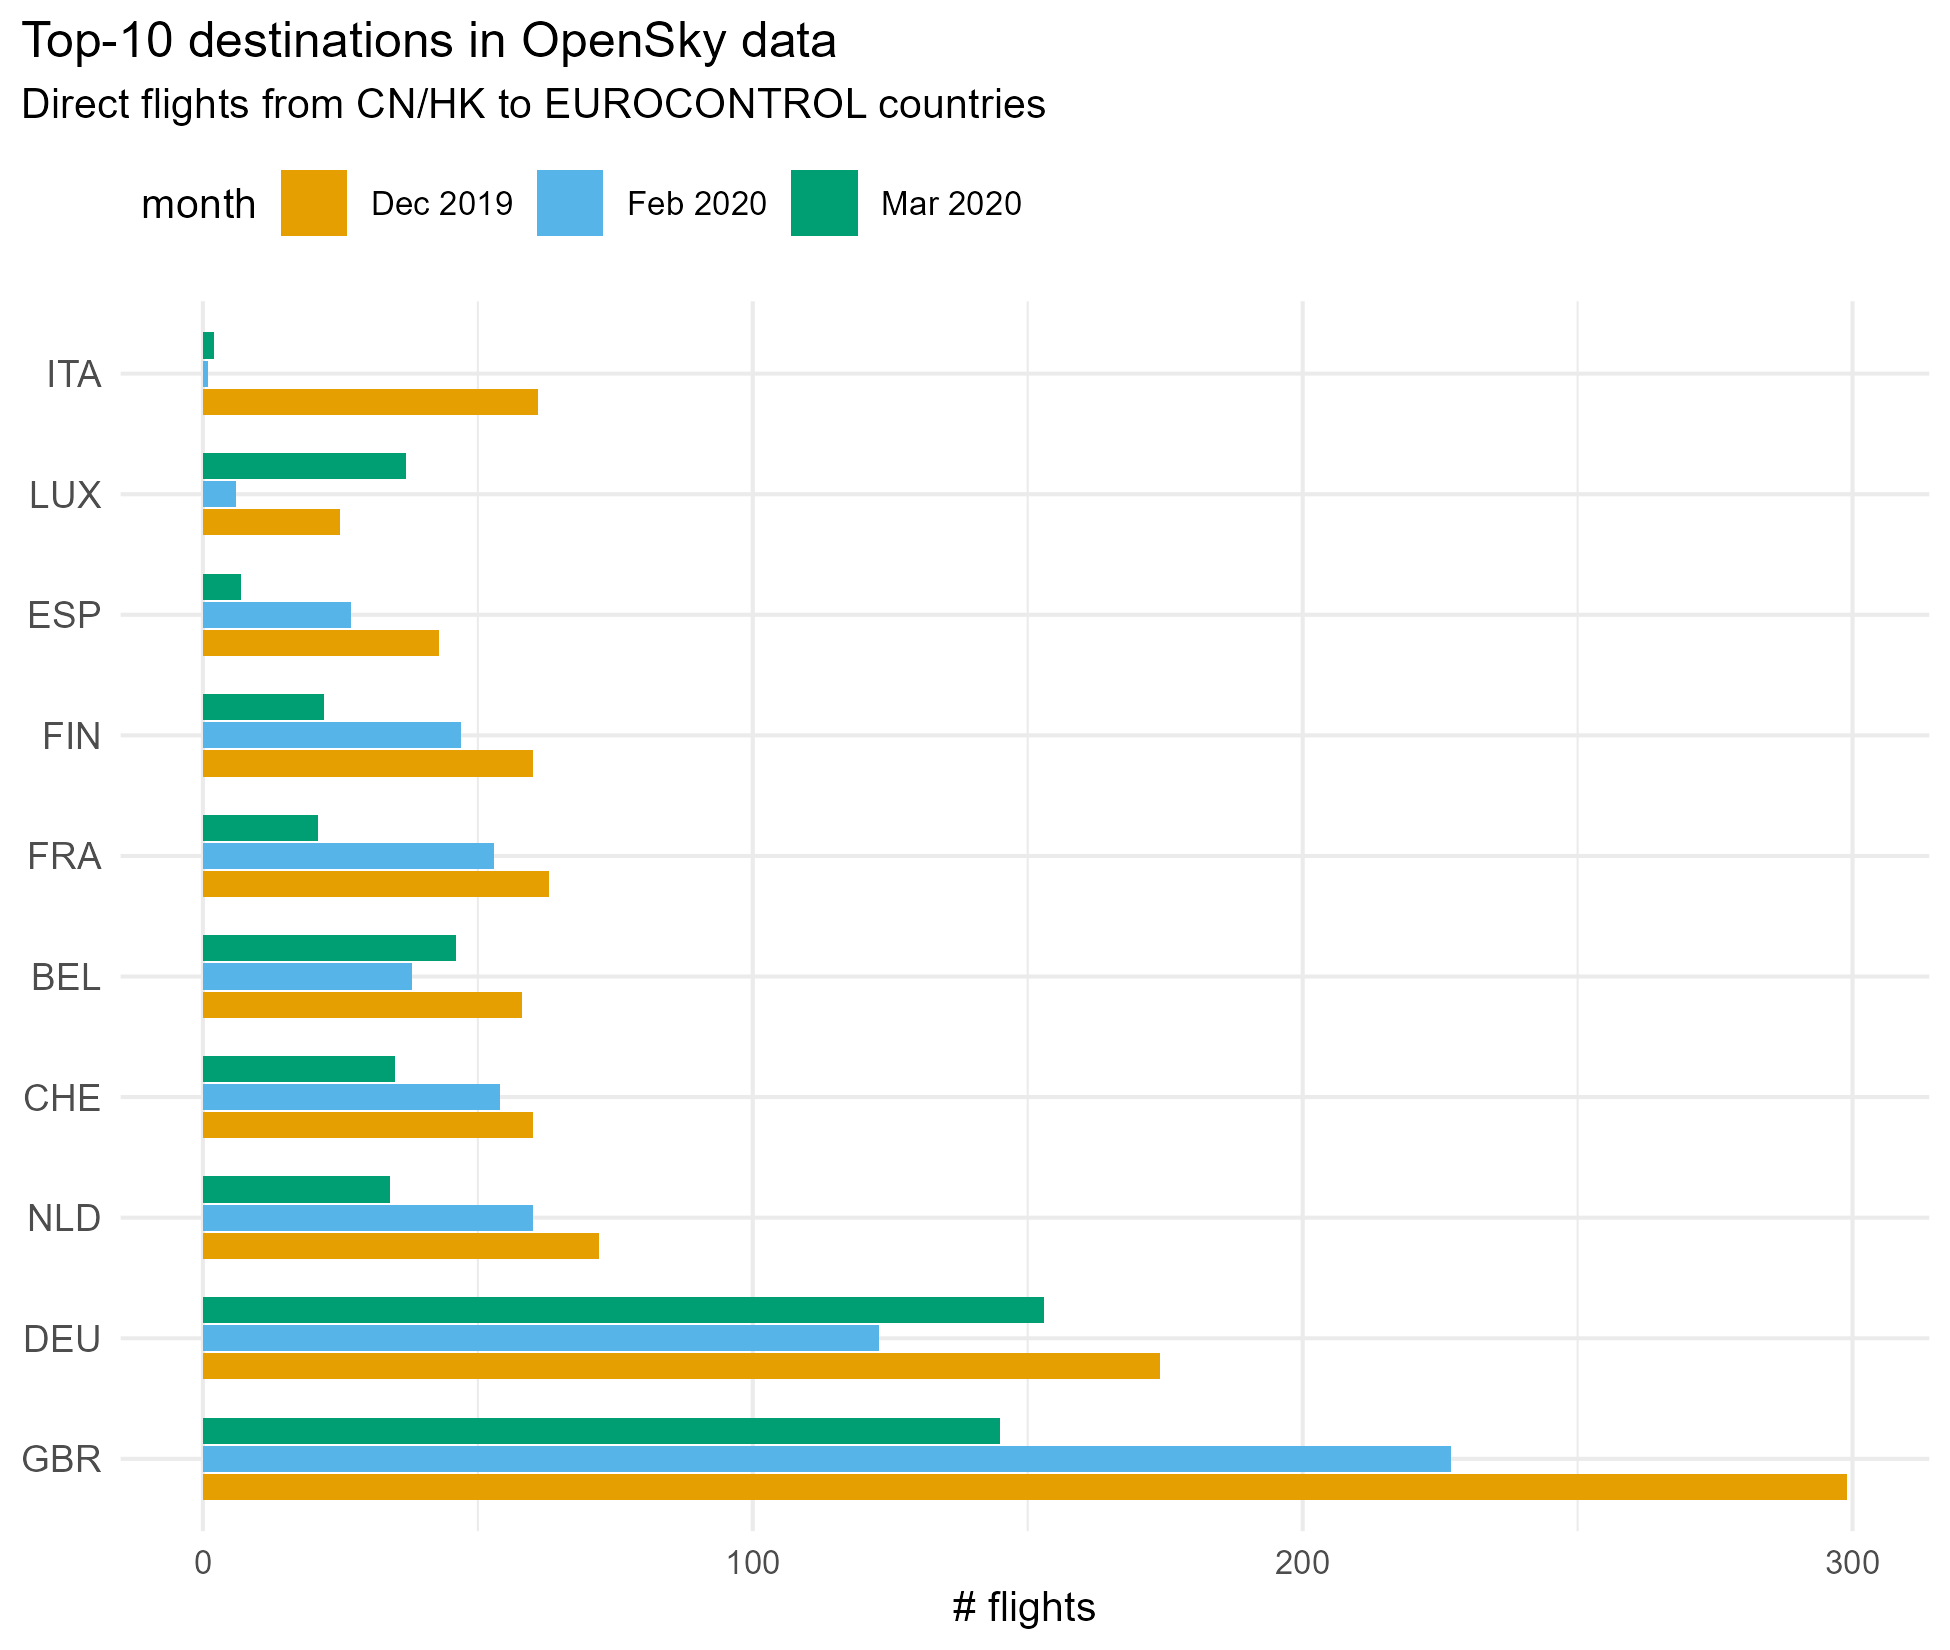
\includegraphics[width=0.9\linewidth,height=\textheight,keepaspectratio]{data/figures/bar_opensky_top10_dec_feb_mar.png}

}

\caption{\label{fig-opensky-bar}Top-10 destinations by number of direct
CN/HK flights in OpenSky data (Dec-2019, Feb-2020, Mar-2020). OpenSky
reflects community ADS-B coverage; patterns motivate prioritising
EUROCONTROL ADRR for exposure measurement.}

\end{figure}%

\clearpage

\subsubsection{Vaccination by exposure quartile (May
2022)}\label{vaccination-by-exposure-quartile-may-2022}

Country membership of flight-exposure quartiles (baseline =
\textbf{Dec-2019 + Mar-2020}; \emph{n} = 25). Quartiles contain 6--7
countries.

\begin{longtable}[]{@{}
  >{\raggedright\arraybackslash}p{(\linewidth - 6\tabcolsep) * \real{0.2810}}
  >{\raggedright\arraybackslash}p{(\linewidth - 6\tabcolsep) * \real{0.2397}}
  >{\raggedright\arraybackslash}p{(\linewidth - 6\tabcolsep) * \real{0.2397}}
  >{\raggedright\arraybackslash}p{(\linewidth - 6\tabcolsep) * \real{0.2397}}@{}}

\caption{\label{tbl-vaccination-quartiles}Country membership of
flight-exposure quartiles (Dec-2019 + Mar-2020 baseline).}

\tabularnewline

\toprule\noalign{}
\begin{minipage}[b]{\linewidth}\raggedright
Q1 (low)
\end{minipage} & \begin{minipage}[b]{\linewidth}\raggedright
Q2
\end{minipage} & \begin{minipage}[b]{\linewidth}\raggedright
Q3
\end{minipage} & \begin{minipage}[b]{\linewidth}\raggedright
Q4 (high)
\end{minipage} \\
\midrule\noalign{}
\endhead
\bottomrule\noalign{}
\endlastfoot
GEO, HRV, IRL, LTU, LUX, LVA, SVK & CZE, GRC, HUN, POL, PRT, SWE & AUT,
CHE, DNK, ESP, FIN, TUR & BEL, DEU, FRA, GBR, ITA, NLD \\

\end{longtable}

For the descriptive comparison in the Discussion,
\texttt{people\_fully\_vaccinated\_per\_hundred} was taken nearest to
\textbf{5 May 2022 (±7 days)} for the same 25-country set
(\texttt{01b\_extract\_vax.R} →
\texttt{data/processed/vax\_snapshot.\{csv,rds\}}). Vaccination figures
are \textbf{not} used in any correlation/regression.





\end{document}
